% !TeX root = ../libro.tex
% !TeX encoding = utf8
\chapter{Fundamentos matemáticos: las SDFs}
Estamos acostumbrados a representar superficies en $\R^3$ a través de ecuaciones paramétricas e implícitas. En el caso de las paramétricas se asigna a cada tupla de parámetros un punto, mientras que para las implícitas, dado un punto la ecuación indica si este se encuentra dentro o fuera de la superficie. El tipo de superficies implícitas más comúnmente estudiado es el de las superficies algebraicas, variedades algebraicas de dimensión dos. Existen varios métodos para la visualización de este tipo de superficies. Uno de ellos es tratar de generar una malla de polígonos previamente a partir de la ecuación para después ser visualizada en tiempo real usando los métodos clásicos. El problema de este método es que no siempre se puede aplicar y conlleva pérdida de precisión en la representación de la superficie. Otro método es el \textit{raytracing}, pero este también puede llegar a perder precisión, además de que es muy lento, haciendo que la representación de una superficie tan simple como una esfera sea computacionalmente muy costoso.\newline

Como solución a esto, T. Sederberg y A.Zundel \cite{Sederberg1989ScanLD} presentaron en 1989 un método para la representación superficies algebraicas sin pérdida de información y de manera eficiente, capaz además de trabajar con siluetas, intersección de curvas y operaciones booleanas. En 1889 John C. Hart \cite{hart2} presenta una técnica de \textit{raymarching} para la representación de fractales usando funciones distancia con signo. Posteriormente, en 1995 \cite{hart} generaliza esta técnica con el uso de \textit{spheretracing} para la representación de cualquier superficie implícita (algebraica o no), punto de partida de este trabajo. Este método nos permitirá representar cualquier superficie en tiempo real con un coste computacionalmente muy bajo y a cualquier nivel de detalle. No obstante, para usarlo debemos comprender qué son las funciones distancia con signo, sus propiedades, y cómo trabajar con ellas.

\begin{definicion}\label{def:sdf}
  Sea $\Omega \subset \R^3$. La \textbf{función distancia} asociada a $\Omega$, que llamamos $d_{\Omega}$ es el campo escalar que a cada punto de $\R^3$ le asigna su menor distancia a la frontera de $\Omega$:
    \begin{align*}
          d_{\Omega} \colon \R^3 &\to \R_0^+,\\
          x &\mapsto \inf\{\Vert x-y\Vert) \colon y \in \delta\Omega\}.
    \end{align*}
    Cuando $\Omega$ sea cerrado, podremos usar el mínimo en lugar del ínfimo.
\end{definicion}

\begin{definicion}\label{d:sdf}
  Sea $\Omega \subset \R^3$. La \textbf{función distancia con signo} asociada a $\Omega$ es el campo escalar de la forma:
  \begin{align*}
          \phi_{\Omega} \colon \R^3 &\to \R,\\
          x &\mapsto \begin{cases}
      d_{\Omega}(x),  &x\in \R^3\setminus \mathring{\Omega}, \\
      -d_{\Omega}(x), &x\in \mathring{\Omega}.
    \end{cases}
    \end{align*}
  En la literatura es común referirse a ellas por sus inglés SDF (\textit{Signed Distance Function}), y la denotaremos simplemente $\phi$ siempre que no haya confusión.
\end{definicion}

 \begin{observacion}
     Un campo escalar $f\colon \R^3\to \R$ cualquiera será una función distancia si existe al menos un $\Omega \subset \R^3$ tal que $f = d_{\Omega}$. De la misma forma, $f$ será una SDF cuando para dicho $\Omega$ se tenga $f=\phi_{\Omega}$.
 \end{observacion}

\begin{definicion}
  Dada una función $\phi\colon \R^3 \to \R$ y $k\in\R$, llamamos \textbf{isosuperficie de $\boldsymbol{\phi}$ con valor $\boldsymbol{k}$} al conjunto:
  \begin{equation*}
      S_{\phi,k} = \{(x,y,z) :  \phi(x,y,z)=k\}.
  \end{equation*}
  Sin pérdida de generalidad podemos suponer $k=0$, pues de no ser el caso, tomamos la función $\phi'(x,y,z)=\phi(x,y,z)-k$ y tenemos que $S_{\phi',0} = S_{\phi,k}$. Por tanto, la denotaremos como $S_\phi$.
\end{definicion}

Nuestra intención es construir una escena definida como la isosuperficie generada por una SDF. A partir de ahora, tomaremos $p=(x,y,z)\in\R^3$.

\begin{ejemplo}\label{ej:sdf}
    Ejemplos simples de SDFs $\phi$ en $p$ para diferentes conjuntos $\Omega$ son:
    \begin{itemize}
        \item \textbf{Esfera de radio $\boldsymbol{r}$ centrada en el origen.}
        \begin{equation*}
            \Omega=\{(x,y,z)\in \R^3 : \Vert (x,y,z)\Vert = r\},\quad \phi(p) = \Vert p\Vert - r.
        \end{equation*}
        \item \textbf{Plano con vector normal unitario $\boldsymbol{n=(a,b,c)}$ y pasando por el origen}.
        \begin{equation*}
            \Omega=\{(x,y,z)\in\R^3 : ax+by+cz = 0\},\quad \phi(p) = p\cdot n.
        \end{equation*}
        \item \textbf{Toro sobre el eje Y de radios $\boldsymbol{R}$ y $\boldsymbol{r}$, con $\boldsymbol{R>r}$}:
        \begin{align*}
            &\Omega=\left\{(x,y,z)\in \R^3 : \left(R-\sqrt{x^2+z^2}\right)^2 + y^2 = r^2\right\},\\[10pt]
            &\phi((x,y,z))= \bigg\Vert (\Vert(x,0,z)\Vert - R, y) \bigg\Vert - r.
        \end{align*}
    \end{itemize}
\end{ejemplo}

\section{Diferenciabilidad}
Antes de seguir avanzando vamos a realizar un estudio de la diferenciabilidad de los SDF, pues nos será de utilidad en las siguientes secciones. Empezamos recordando varios conceptos de análisis diferencial \cite{diff} fijadas las variables $\{x_1,x_2,x_3\}$ y la base usual $$B=\{e_1,e_2,e_3\} = \{(1,0,0),(0,1,0),(0,0,1)\}.$$

Cuando sea conveniente identificaremos
\begin{equation*}
    x_1=x,\quad x_2=y,\quad x_3 = z.
\end{equation*}

\begin{definicion}\label{def:parcial}
    Sea $U$ un abierto de $\R^3$ y $\phi: U \to \R$. Para $i\in \{1,2,3\}$, definimos la \textbf{$\boldsymbol{i}$-ésima derivada parcial} de $\phi$ en $p_0\in\R^3$ como
    \begin{equation*}
        \frac{\partial \phi}{\partial x_i}(p_0) = \lim_{h\to 0}\frac{\phi(p_0+he_i) - \phi(p_0)}{h}.
    \end{equation*}
\end{definicion}

\begin{definicion}
    Sea $U$ un abierto de $\R^3$ y $\phi: U \to \R$. Diremos que $\phi$ es \textbf{diferenciable} en $p_0 \in U$ si existen todas sus derivadas parciales en $p_0$ y son continuas. Definimos la \textbf{diferencial} de $\phi$ en $p_0$ como la suma de todas sus parciales en dicho punto, y la denotamos como $d\phi(p_0)$.

    % \begin{equation*}
    %     \text{lím}_{p\to p_0} \frac{\phi(p)-\phi(p_0) - \nabla\phi(p_0)\cdot(p-p_0)}{\Vert p-p_0\Vert} = 0.
    % \end{equation*}
\end{definicion}

\begin{definicion}
    Dado un abierto $U\subseteq \R^3$, diremos que la \textbf{clase de diferenciabilidad} de una función $\phi:U\to \R$ es $\mathbb{C}^n(U)$ si para $i\in \{1,2,3\}$ y $j\in \{0,\dots, n\}$ existen y son continuas todas las parciales
    \begin{equation*}
        \frac{\partial^j \phi}{\partial x_i}(p),\ \text{para todo } p\in U.
    \end{equation*}
\end{definicion}

\begin{definicion}
  Llamamos \textbf{gradiente} de $\phi\colon \R^3\to\R$ a la función
  \begin{align*}
      \nabla\phi\colon \R^3 &\to \R^3,\\
      p &\mapsto \left(\frac{\partial \phi}{\partial x_1}(p), \frac{\partial \phi}{\partial x_2}(p), \frac{\partial \phi}{\partial x_3}(p)\right).
  \end{align*}
\end{definicion}

\begin{definicion}
  Dada $\phi:\R^3\to \R$ diferenciable, definimos la \textbf{derivada direccional} en $p_0\in \R^3$ en la dirección $v\in\R^3$ a:
  \begin{equation*}
    \nabla_v \phi(p_0) = \nabla \phi(p_0) \cdot v = \frac{\partial{\phi}(p_0)}{\partial{x}}v_x + \frac{\partial{\phi}(p_0)}{\partial{y}}v_y + \frac{\partial{\phi}(p_0)}{\partial{z}}v_z.
  \end{equation*}
\end{definicion}




Ahora mismo, dado un SDF arbitrario no tenemos información alguna sobre su diferenciabilidad, ya que su expresión puede ser de lo más variada y compleja. Veamos una propiedad que cumplen todos los SDF y que nos permitirá obtener algo de información al respecto \cite{lips,derivWiki}.

\begin{definicion}
    Una campo escalar $\phi\colon \R^3 \to \R$ se dice \textbf{lipschitziano} si existe una constante $L>0$ tal que
    \begin{equation*}
        \vert \phi(p)-\phi(q)\vert \le L\Vert p-q\Vert,\ \text{para todo } p,q\in \R^3.
    \end{equation*}
    La constante $L$ recibe el nombre de \textbf{constante de Lipschitz}.
\end{definicion}

\begin{proposicion}
    Sea $\phi\colon \R^3 \to \R$ una función lipschitziana cualquiera con constante de Lipschitz $L$. Entonces
    \begin{equation*}
        \vert d\phi(p)\vert \le L
    \end{equation*}
    en todo punto donde sea diferenciable.
\end{proposicion}

\begin{lema}
    Sea $\phi:\R^3\to \R$ la función distancia con signo asociada a $\Omega$. Entonces $\phi$ es lipschitziana con constante $L=1$.
\end{lema}
\begin{proof}
    Sean $p$ y $q\in \R^3$. Usando la \autoref{def:sdf}, para todo $s\in \delta\Omega$ se tiene
    \begin{equation*}
        \phi(p) \le \Vert p-s\Vert = \Vert p-q+q+s\Vert \le \Vert p-q\Vert + \Vert q-s\Vert.
    \end{equation*}
    Por tanto, $\phi_{\Omega}(p) - \Vert p-q\Vert \le \Vert q-s \Vert$, luego $\phi_{\Omega}(p) - \Vert p-q\Vert \le \Inf_{s\in \delta\Omega}(\Vert q-s \Vert) = \phi_{\Omega}(q)$ y obtenemos
    \begin{equation*}
         \phi_{\Omega}(p) - \phi_{\Omega}(q) \le \Vert p-q \Vert.
    \end{equation*}
    De forma análoga podemos ver que $\phi_{\Omega}(q) - \phi_{\Omega}(p) \le \Vert q-p \Vert$, concluyendo que
    \begin{equation*}
        \vert \phi_{\Omega}(p) - \phi_{\Omega}(q)\vert \le 1\cdot \Vert p-q\Vert.\qedhere
    \end{equation*}
\end{proof}

\begin{lema}[Teorema de Rademacher]
    Sea $U$ un abierto de $\R^3$ y $\phi:U\to \R$ lipschitziana. Entonces $\phi$ es diferenciable en casi todo punto de $U$.
\end{lema}

Tenemos por tanto asegurado que $\phi_{\Omega}$ será diferenciable en casi todo punto de $\R^3$. No obstante, podemos concretar aún más dónde están los puntos de conflicto cuando $\Omega$ sea lo suficientemente regular \cite{dif1,dif2}. Para ello necesitaremos introducir el concepto de esqueleto de una superficie \cite{derivWiki}.
\begin{definicion}
    Sea $\phi_{\Omega} \colon \R^3\to \R$ un SDF. Llamamos \textbf{esqueleto} de $\Omega$ al conjunto de puntos de $\R^3$ cuya distancia a la superficie puede obtenerse como la distancia a dos o más puntos distintos de $\delta \Omega$:
    \begin{equation}
        \epsilon(\Omega) = \{p\in \R^3 : \phi_{\Omega}(p) = \Vert p-q\Vert = \Vert p-r\Vert,\ q,r\in \delta\Omega ,\ q\neq r \}.
    \end{equation}
\end{definicion}

\begin{definicion}
    Sea $\Omega \subset \R^3$ y $p\in \Omega$. Llamamos \textbf{vector normal} en $p$ al vector de norma uno y perpendicular al borde de $\Omega$ en $p$. Lo denotamos $N_p$.
\end{definicion}

\begin{definicion}
    Decimos que $\Omega \subseteq \R^3$ es \textbf{regular} si para cada $p\in \Omega$ existen abiertos $U\subseteq \R^2$ y $V\subseteq \R^3$ junto a una aplicación $\psi\colon U \to V\cap \Omega$ tal que:
    \begin{enumerate}
        \item $\psi$ es un homeomorfismo, es decir, es continua, biyectiva y con inversa continua,
        \item $\psi$ es diferenciable y su diferencial es inyectiva.
    \end{enumerate}
\end{definicion}

El siguiente teorema, cuya demostración podemos consultar en \cite{dif1}, nos proporciona una caracterización geométrica de la diferenciabilidad de cualquier distancia con signo bajo $\phi_{\Omega}$ ciertas hipótesis de regularidad para $\Omega$.
\begin{teorema}\label{teo:diff}
    Sea $\Omega \subseteq \R^3$ cuya frontera es regular y $\phi_{\Omega} \colon \R^3\to \R$ la función distancia con signo asociada a $\Omega$. Entonces $\phi_{\Omega}$ es diferenciable en un entorno tubular $U$ de $\delta \Omega$. Es más, para cada $p\in \R^3$ se cumple una se las siguientes propiedades:
    \begin{enumerate}
        \item $p\in \delta \Omega$ y $\phi_{\Omega}$ es diferenciable en $p$ con $\nabla S_{\phi(p)} = N_p$,
        \item $p\notin \delta \Omega$ y $\phi_{\Omega}$ es diferenciable en $p$ si y sólo si $p\in \R^3\setminus \epsilon(\Omega)$, en cuyo caso
        \begin{equation*}
            \nabla \phi_{\Omega}(p) = \frac{q-p}{\phi_{\Omega}(p)},
        \end{equation*}
        donde $q$ es el único punto de $\delta\Omega$ tal que $\phi_{\Omega}(p) = \Vert q-p\Vert$.
    \end{enumerate}
\end{teorema}

\begin{corolario}
    Todo SDF $\phi\colon \R^3\to \R$ satisface la ecuación de la eikonal 
    \begin{equation*}
        \Vert \nabla \phi(p)\Vert = 1
    \end{equation*}
    en todo punto $p$ donde sea diferenciable.
\end{corolario}
% A la vista de este resultado podemos diferenciar $\phi$ con tranquilidad, pues solo estamos interesados en estudiar el gradiente en puntos de $\delta\Omega$, luego
% \begin{equation*}
    
% \end{equation*}

% TODO: ver si decir que podria calcularse fuera del shader pasanndo el string al shader y recompilando. Si no, ver si comentar algo de que hay que calcularlo cada frame, y por eso no podemos hacerlo analiticamente
% De ser derivable, podría ser una buena opción calcular el gradiente una única vez al momento de definir $\phi$, tras lo cual para obtener $N$ solo habría que realizar evaluaciones de dicho gradiente. Sin embargo, esto requeriría de varias comprobaciones previas, y aún necesitaríamos otro método para tratar las no diferenciables. Por ello nos decantaremos por un método numérico más sencillo que únicamente hará uso de evaluaciones de $\phi$.



\section{Funciones cota de distancia}
Hemos visto que las funciones distancia con signo nos proporcionan la distancia signada exacta en cada punto al más cercano de un conjunto $\Omega\subset \R^3$, pero lo cierto es que para representar las isosuperficies que generan no se necesita tanta precisión, ya que mientras dos funciones tengan los mismos ceros generarán la misma isosuperficie. Sin embargo, para representar la superficie en las siguientes secciones usaremos el método de \textit{spheretracing} (\autoref{sec:tracing}), que sí utiliza la información de la distancia en puntos diferentes a la frontera de $\Omega$. Introducimos un concepto que nos permitirá seguir usando este método pero no es tan restrictivo como el de función distancia con signo \cite{hart}.

\begin{definicion}
    Sea $\Omega\subset \R^3$ y $\phi$ su SDF. Una \textbf{cota de la distancia con signo} asociada a $\Omega$ es un campo escalar $\gamma\colon \R^3\to \R$ cumpliendo
    \begin{equation*}
        \vert \gamma(p)\vert \le \vert \phi(p)\vert,\ \text{ para todo } p\in\R^3,
    \end{equation*}
    y que tiene el mismo signo que $\phi$ en cada punto. En su artículo \cite{hart2}, C. Hart se refiere a ellas como SDB (\textit{Signed Distance Bound}).
\end{definicion}

Observamos que una SDF es un caso especial de SDB en el que se cumple la igualdad de la definición anterior, y que si ambos tipos de funciones están asociadas a un mismo $\Omega$ tendrán los mismos ceros, generando por tanto la misma isosuperficie. Aunque trabajar con una función cota de distancia en \textit{spheretracing} hará que la convergencia sea más lenta al proporcionar una cota más conservativa, en muchos casos será también más rápida de evaluar que una función distancia con signo por tener una expresión más simple, haciendo que sea deseable trabajar con ellas. Habrá otras ocasiones en las que incluso será imposible obtener una función distancia signada para un cierto $\Omega$. Por estos motivos en la literatura no se suele distinguir entre función distancia con signo y función cota de distancia, y como mucho se utilizan los términos función distancia exacta y aproximada respectivamente cuando se quiere realizar una distinción.\newline

Veamos algunos ejemplos de funciones distancia aproximadas.
\begin{ejemplo}\label{ej:sdf}
    Para los siguientes conjuntos $\Omega$ podemos definir las funciones distancia aproximadas:
    \begin{itemize}
        \item \textbf{Cono centrado en el origen a lo largo del eje Y con altura $\boldsymbol{h}$ y ángulo $\theta$.}
        \begin{align*}
            &\Omega=\{(x,y,z)\in \R^3 : (x^2+z^2)(\cos\theta)^2 - y^2(\sin\theta)^2\},\\[8pt]
            &\phi((x,y,z)) = \Max\Big((\sin\theta, \cos\theta)\cdot (\Vert (x,0,z)\Vert, y), -h-y\Big).
        \end{align*}
        \item \textbf{Elipsoide fijados $\boldsymbol{a,b,c\in \R\setminus \{0\}}$}.
        \begin{align*}
            &\Omega=\left\{(x,y,z)\in\R^3 : \frac{x^2}{a^2}+\frac{y^2}{b^2}+\frac{z^2}{c^2} = 0\right\},\\[10pt]
            &\phi((x,y,z)) = \Big\Vert \left( \frac{x}{a},\frac{y}{b},\frac{z}{c} \right) \Big\Vert \cdot \left(  \Big\Vert \left( \frac{x}{a},\frac{y}{b},\frac{z}{c} \right) \Big\Vert -1\right)\ \Big{/}\ \Big\Vert \left( \frac{x}{a^2},\frac{y}{b^2},\frac{z}{c^2} \right) \Big\Vert .
        \end{align*}
    \end{itemize}
\end{ejemplo}


\section{Operaciones sobre SDF}\label{sec:operaciones}

Si bien estas primitivas son fáciles de generar, también son muy simples y nos serán insuficientes si queremos construir escenas más complejas. Como comentamos en la introducción, una de las principales ventajas del uso de ecuaciones implícitas para representar modelos geométricos es la facilidad de combinación de estas primitivas, por ejemplo mediante operaciones booleanas o deformaciones. Sin embargo los sistemas que hacían uso de esta técnica no estaban lo suficientemente estructurados como para permitir aplicar estas operaciones de manera general e intuitiva, haciendo que no se pudieran aplicar de forma local y por tanto no se pudieran generar escenas complejas.\newline


Esto cambió en 1999 con el artículo de B. Wyvill y otros \cite{blobtree}, en el que sugieren usar una estructura de árbol para definir modelos como combinación de otros a través de operaciones básicas. La gran ventaja de este método es que es muy extensible, y además permite ver de forma muy clara la estructura del modelo. En esta sección estudiaremos los principales tipos de estas operaciones.

\subsection{Operaciones booleanas}
Una de las técnicas más útiles para generar nuevas formas a partir de primitivas es la geometría de sólidos constructiva. Por la naturaleza de las SDFs, estas operaciones se implementan fácilmente usando las funciones máximo y mínimo.

\begin{definicion}[Operaciones Booleanas]\label{p:boolean}
    Sean $A$ y $B$ isosuperficies generadas por $\phi$ y $\gamma$ respectivamente. La función $\mu$ define la isosuperficie para las siguientes operaciones.
    \begin{itemize}
        \item \textbf{Unión: } $\mu_{A\cup B}(p) = \Min(\phi(p), \gamma(p))$.
        \item \textbf{Intersección: } $\mu_{A\cap B}(p) = \Max(\phi(p), \gamma(p))$.
        \item \textbf{Diferencia: } $\mu_{A\setminus B}(p) = \Max(\phi(p), -\gamma(p))$.
    \end{itemize}
\end{definicion}

Solo en el caso de la unión se obtiene una SDF exacta, ya que al aplicar la función máximo en el interior de la superficie (donde $\phi(p) < 0$) el resultado puede ser solo una cota inferior de la distancia. En nuestro caso solo estamos interesados en visualizar la frontera de las superficies así que podemos obviar este problema, con la salvedad de que el algoritmo de \textit{spheretracing} requiera de más iteraciones.\newline

Un problema de usar estas transformaciones es que produce discontinuidades en la derivada de la función resultante. Trataremos de evitar esta situación, además de por motivos analíticos, por motivos visuales, ya que esto produce bordes muy acusados en la intersección de ambas superficies. Existen muchas formas de combinar funciones distancia de forma más natural. Usaremos una de las más extendidas, usada por programas de modelado 3D como Blender \cite{repo:blender} o videojuegos como Dreams \cite{game:dreams}, y que ha sido estudiada por Íñigo Quílez en su web \cite{article:smooth}.

\begin{observacion}
    Para mayor claridad del razonamiento, en las figuras se representarán funciones de variable real, a pesar de que nosotros trabajamos en $\R^3$.
\end{observacion}

Explicaremos la técnica poniendo como ejemplo la unión, y al final veremos como la intersección y la diferencia se deducen fácilmente de esta. La idea es, dadas $\phi$ y $\gamma$, añadir una corrección para cada punto a la función mínimo original para que cumpla ciertos requisitos. Por comodidad, definiremos 
\begin{align*}
      \Min_{\phi,\gamma}\colon \R^3 &\to \R,\\
      p &\mapsto \Min(\phi(p),\gamma(p)).
\end{align*}

Llamaremos a la mencionada corrección $\omega_k\colon \R^3\to\R$, donde $k\in \R_0^+$ es un coeficiente que controlará la intensidad del suavizado. Por tanto, la versión suavizada de la función mínimo original será
\begin{align*}
      \smin_{\phi,\gamma}\colon \R^3 &\to \R,\\
      p &\mapsto \Min_{\phi,\gamma}(p) - \omega_k(p).
\end{align*}

Como no queremos que este cambio afecte al algoritmo de \textit{spheretracing}, debemos asegurar que se cumpla $\Min_{\phi,\gamma}(p)\ge \smin_{\phi,\gamma}(p)$, esto es,
\begin{equation*}
\omega_k(p)\ge 0,\ \text{para todo } p\in \R^3,\ \text{para todo } k\in \R^+_0.
\end{equation*}

Si estudiamos cómo se comporta la versión real de la función mínimo en la \autoref{fig:min_real}, vemos que los puntos de conflicto se encuentran cerca de las intersecciones de las gráficas de $\phi$ y $\gamma$, es decir, cuando $\phi$ y $\gamma$ están arbitrariamente cerca. En el resto de puntos no queremos modificar la función original, luego estudiaremos el comportamiento de $\smin$ en el conjunto de entornos de las intersecciones. Usaremos el valor de $k$ para decidir el tamaño de estos entornos, aplicando la corrección únicamente en los puntos del conjunto
\begin{equation*}
    B_{k} = \{p\in\R^3 : |\phi(p)-\gamma(p)| \le k\},
\end{equation*}
de forma que $\omega(p) = 0$ cuando $p\notin B_{k}$.\newline

\begin{figure}[t]
    \centering
    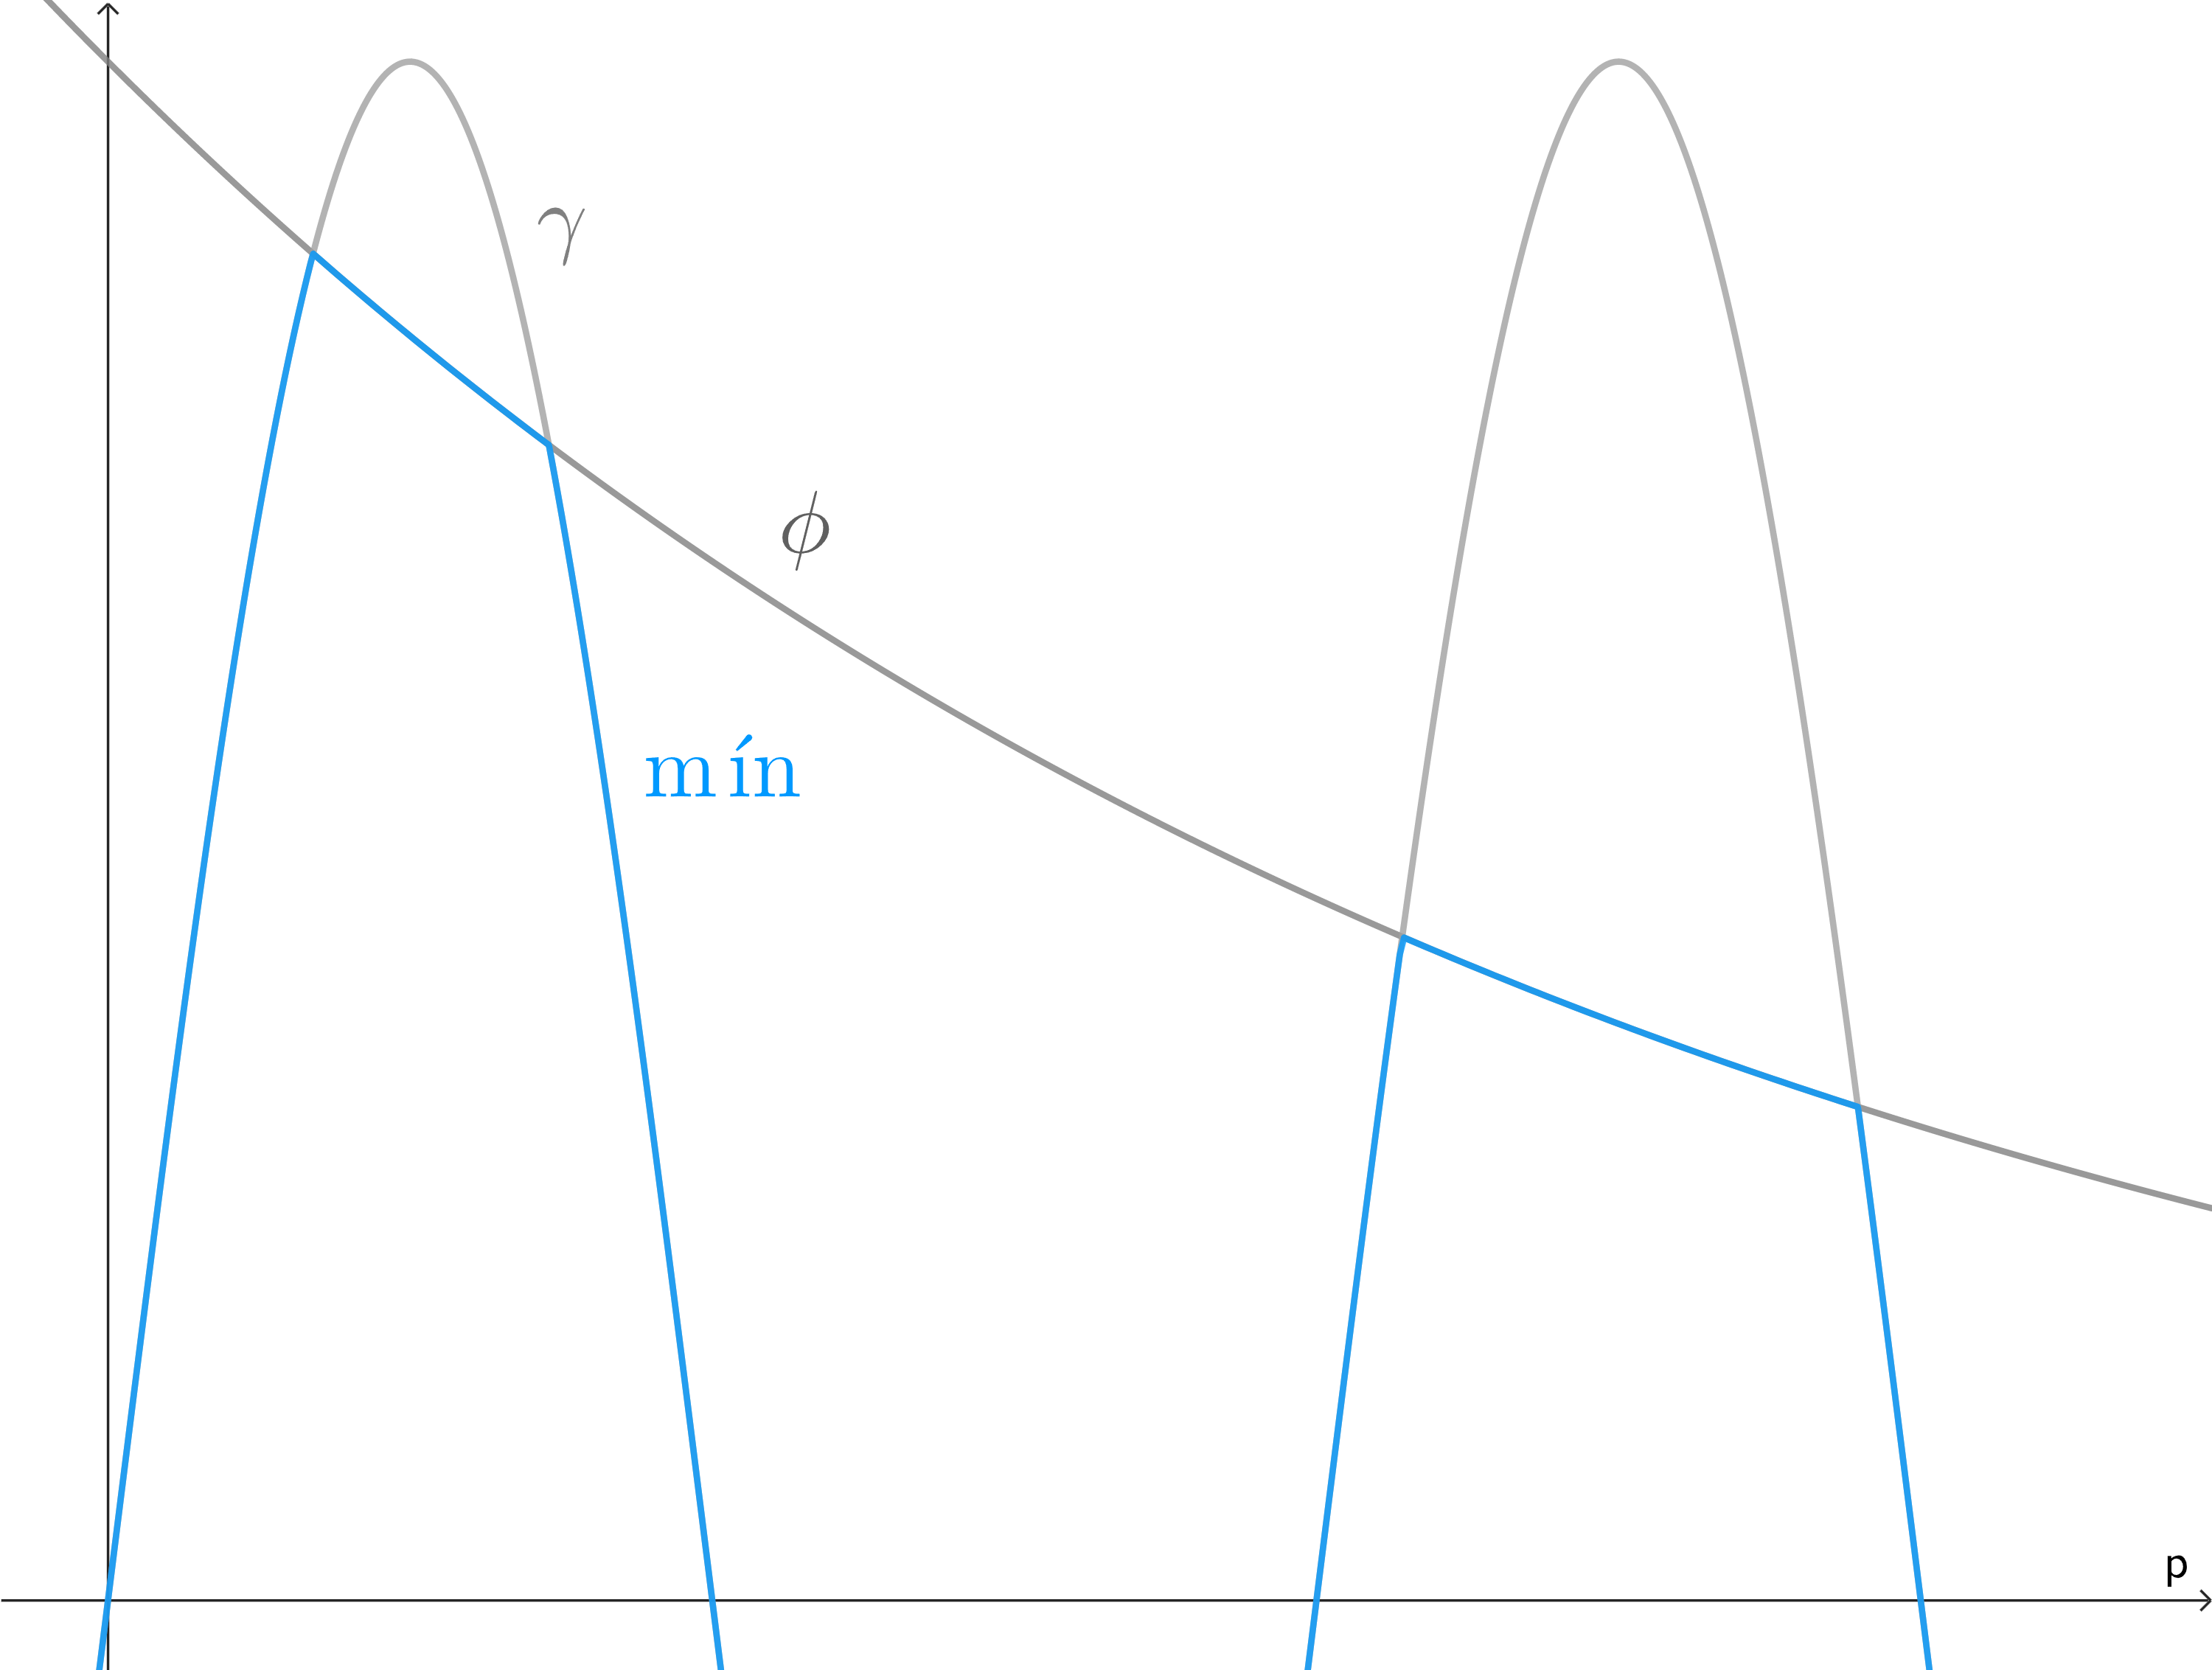
\includegraphics[width=0.75\textwidth]{Plantilla-TFG-master/img/smooth_real.png}
    \caption{Gráfica de $\Min\colon \R\to\R$}
    \label{fig:min_real}
\end{figure}

Para asegurar que $\smin$ sea continua en la frontera de $B_{k}$, imponemos la condición 
\begin{equation*}
    \omega_k(p) = 0,\ \text{para todo } p \in \delta B_{k}.
\end{equation*}
Por otro lado, es lógico que $\omega_k$ tenga su mayor influencia justo en las intersecciones, luego imponemos también 
\begin{equation*}
    \omega_k(c) = s, \text{ donde } c \in I = \{p\in\R^3 : \phi(p) = \gamma(p)\},\ s\in \R.
\end{equation*}

El valor $s$ es el que deberemos ajustar para que $\smin$ cumpla nuestros requisitos. Fijado un $p\in B_{k}$, consideramos una primera aproximación para $\omega_k$ :
\begin{equation*}
    \omega_k(p) = s\left( 1-\frac{|\phi(p)-\gamma(p)|}{k} \right)^n = \begin{cases}
        s\left( 1-\frac{\phi(p)-\gamma(p)}{k}\right)^n,\ \phi(p)>\gamma(p), \\[10pt]
        s\left( 1+\frac{\phi(p)-\gamma(p)}{k}\right)^n,\ \phi(p)\le \gamma(p)\\[10pt]
    \end{cases}  ,\ s\in\R,\ n\in\N,
\end{equation*}
donde hemos añadido el parámetro $n$ para añadir más control sobre el resultado final.\newline 
\begin{figure}[!h]
     \begin{minipage}[c]{0.49\linewidth}
        \centering
        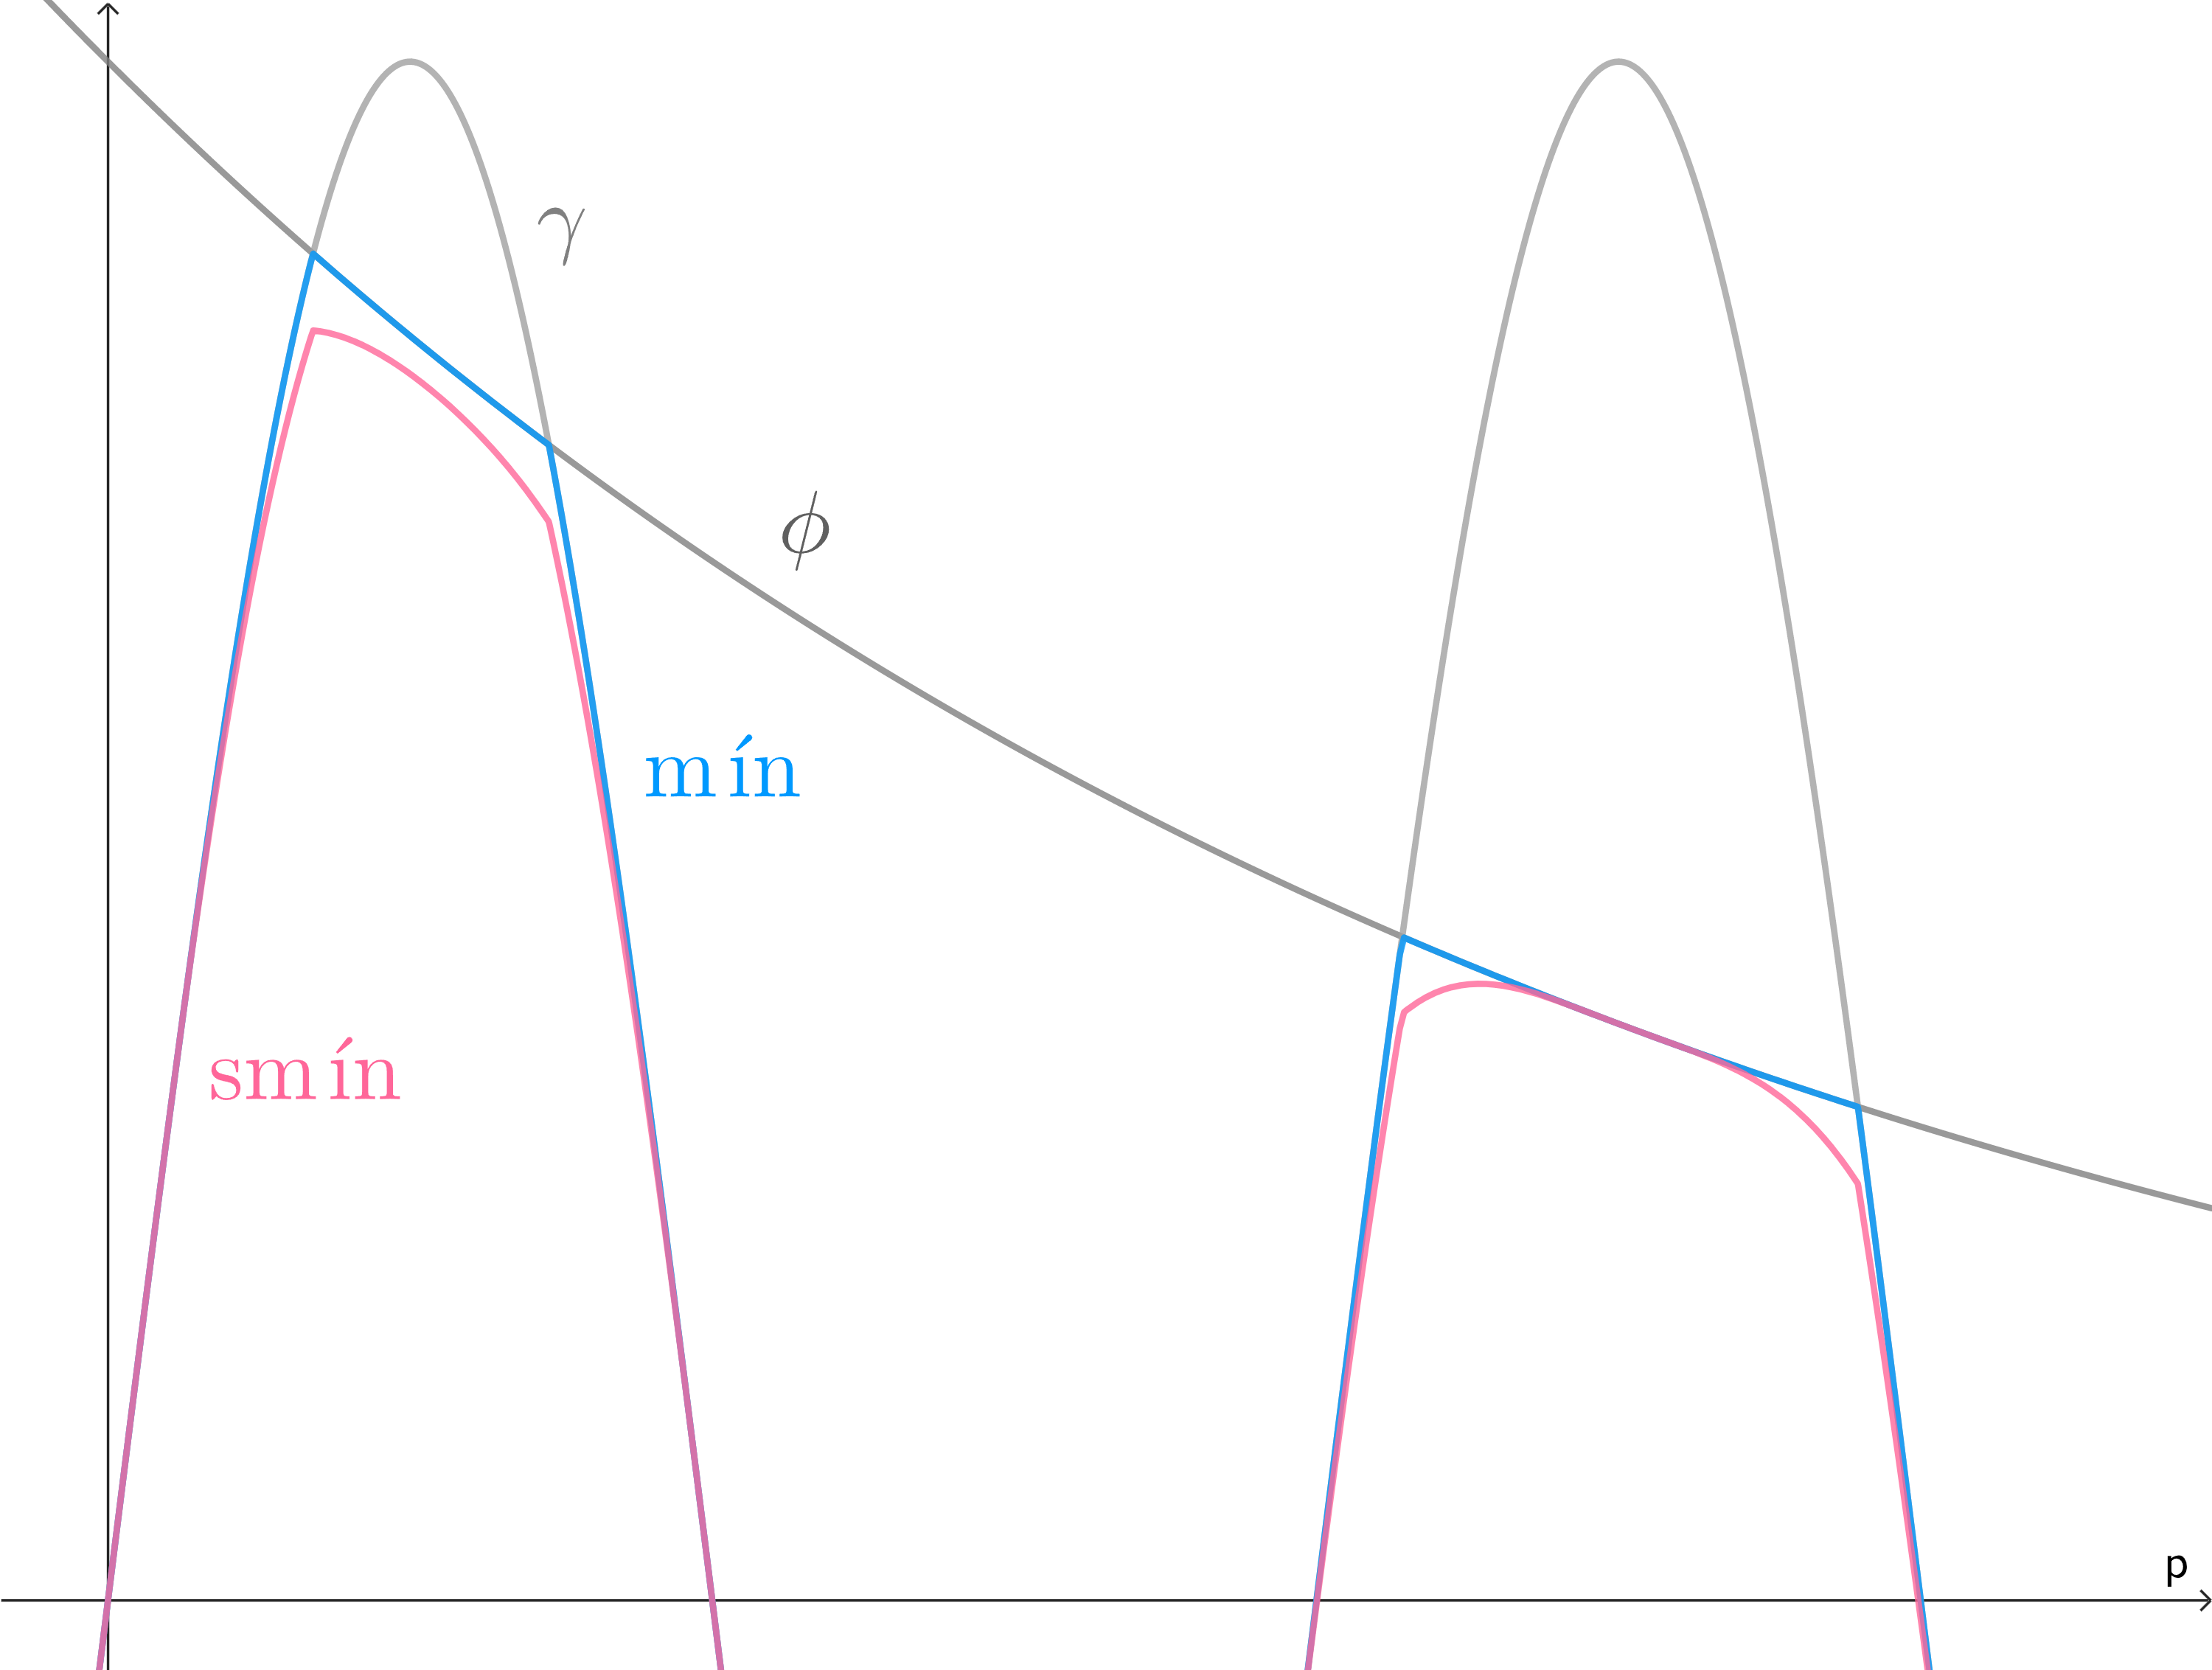
\includegraphics[width=0.95\textwidth]{Plantilla-TFG-master/img/smin_1.png}
        \caption{$k=0.6$}
     \end{minipage}
     \begin{minipage}[c]{0.49\linewidth}
        \centering
        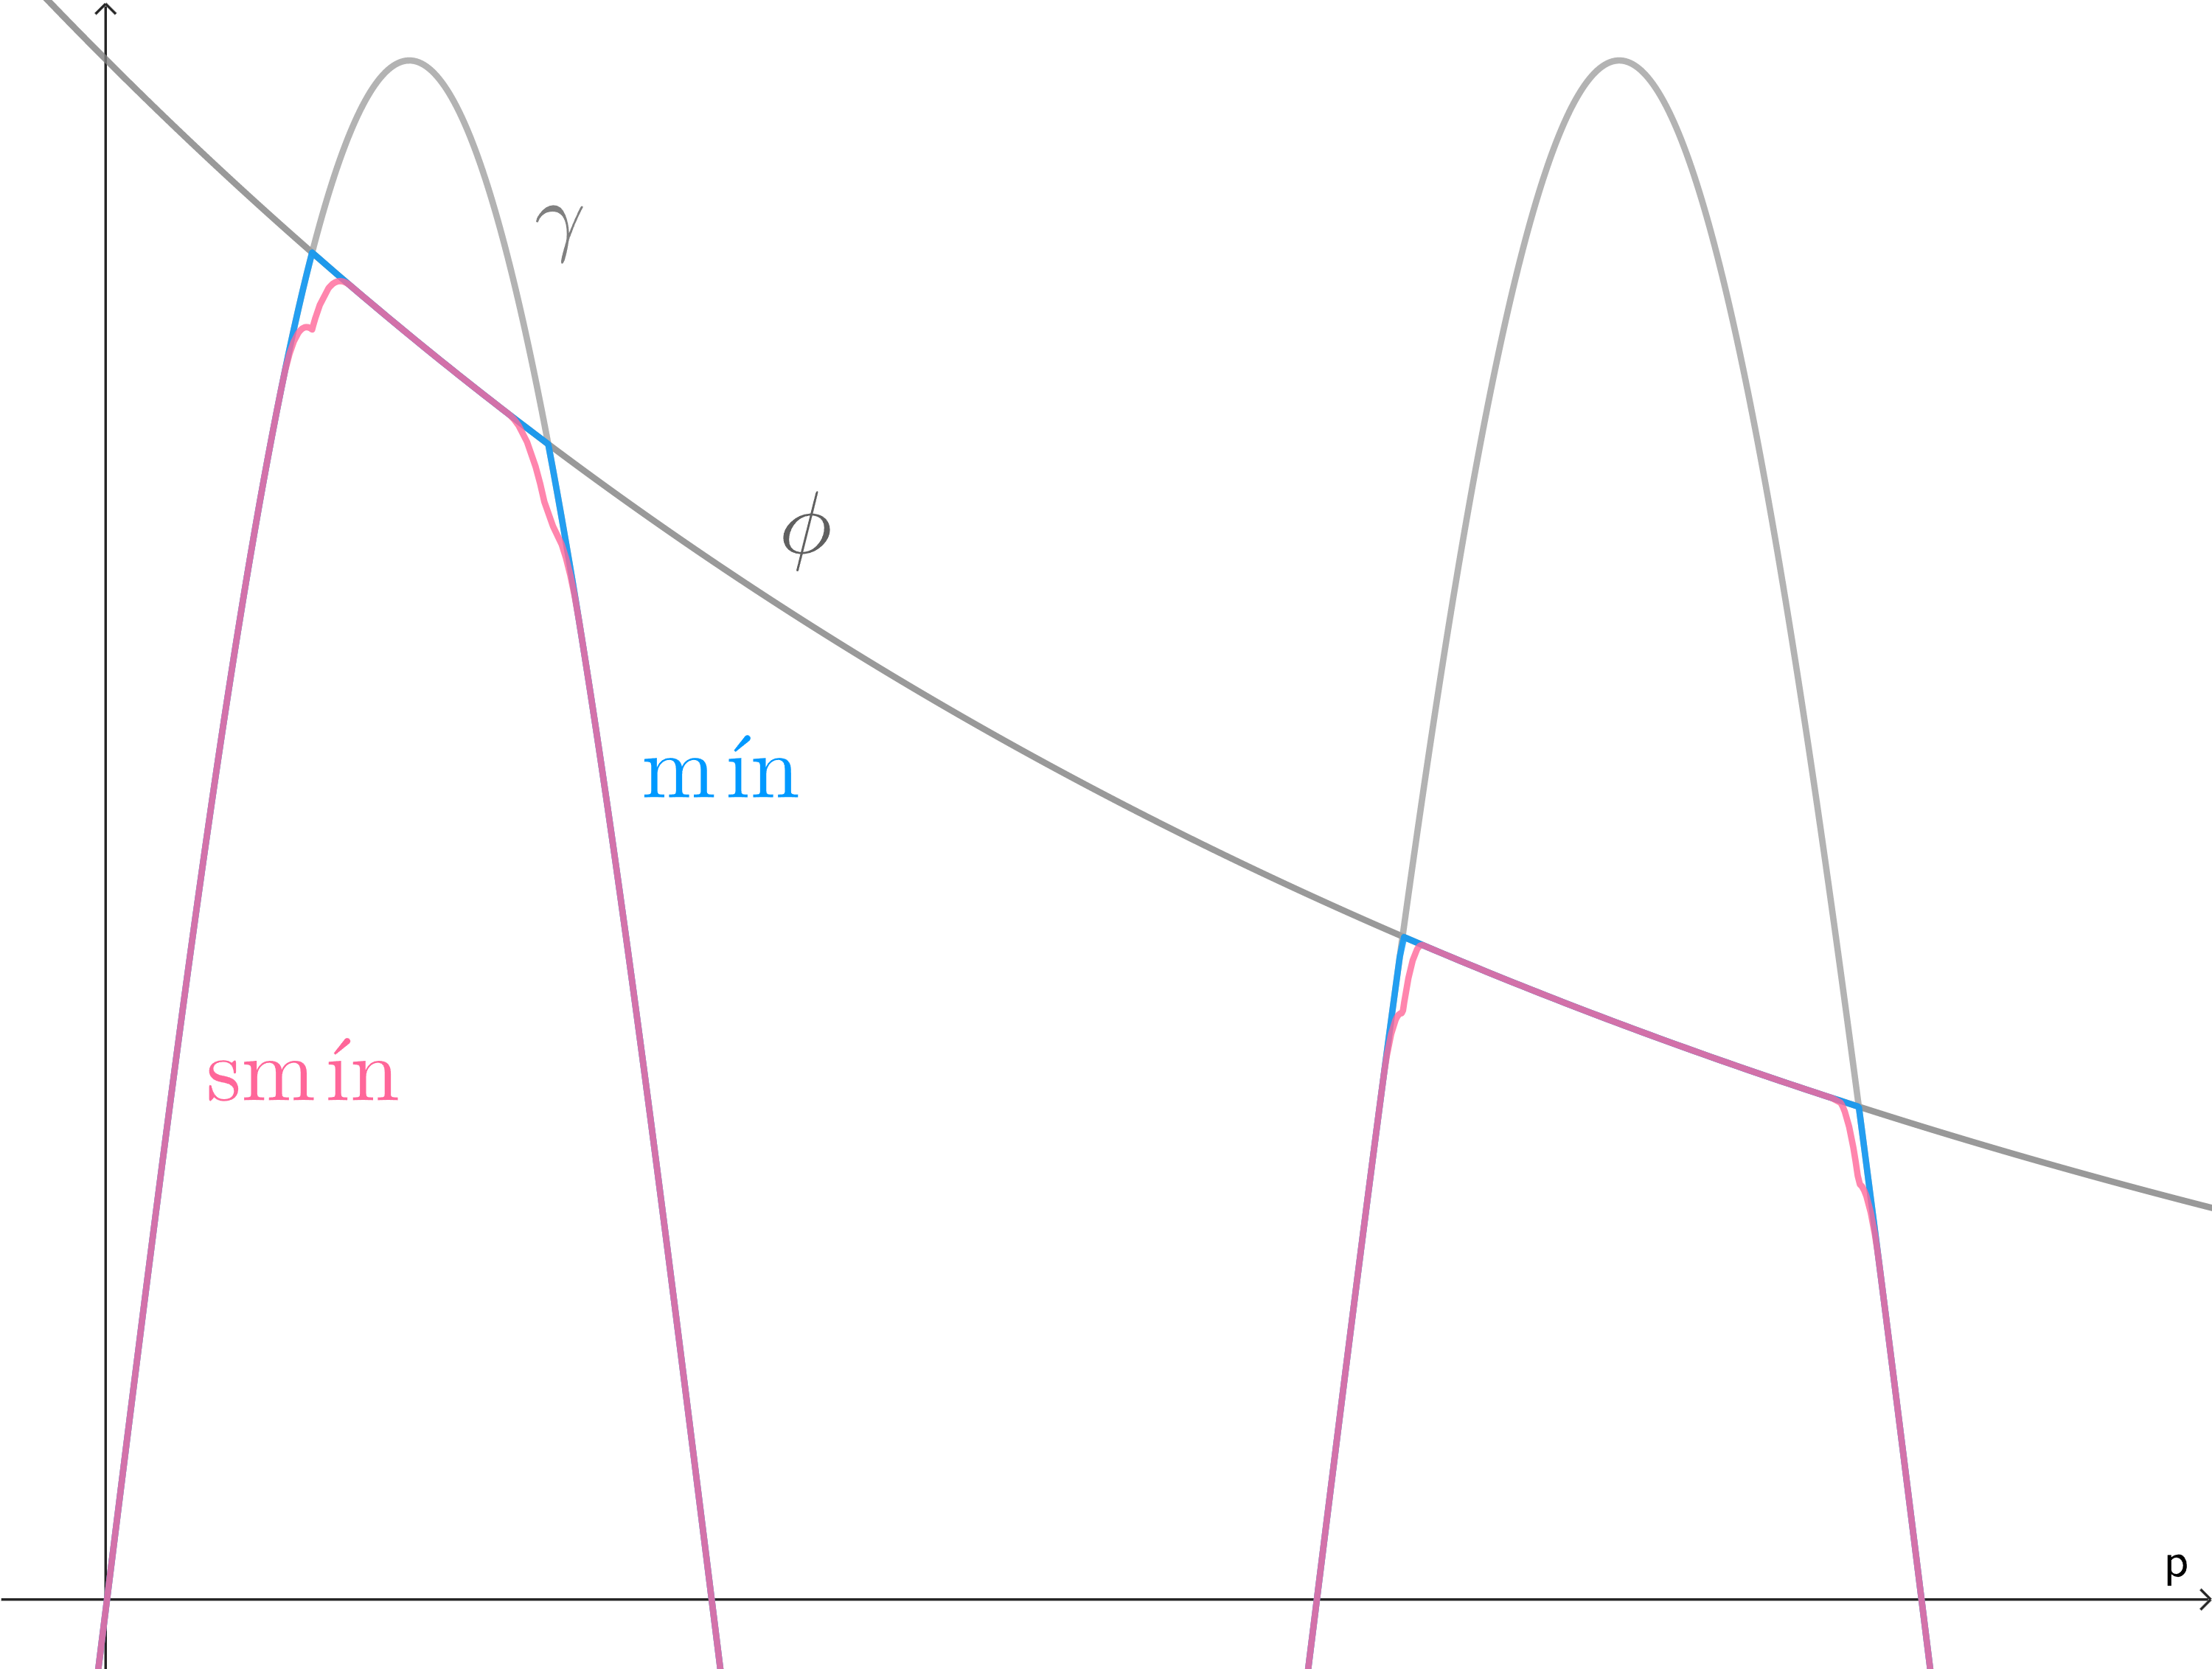
\includegraphics[width=0.95\textwidth]{Plantilla-TFG-master/img/smin_2.png}
        \caption{$k=0.1$}
     \end{minipage}
     \caption{Primera aproximación de $smin(p)$ con $s=0.05$ y $n=2$}
     \label{fig:smooth1}
\end{figure}

Nuestro objetivo es que $\smin$ tenga un aspecto natural y varíe de forma suave. Comprobemos las propiedades que debería cumplir $\smin$ para ser $\mathcal{C}^1$ en cada entorno de $B_k$. Que es continua es evidente:
\begin{equation*}
    \phi(p)=\gamma(p), \text{ luego } \frac{\phi(p)-\gamma(p)}{k} = 0, \text{ y por tanto } \omega_k(p) = s.
\end{equation*}

Otra condición necesaria es que sus derivadas parciales sean continuas. Para todo $i\in \{1,2,3\}$, estas son de la forma
\begin{align*}
    \frac{\partial \smin}{\partial x_i}(p) &= \begin{cases}
        \frac{\partial \gamma}{\partial x_i}(p)+ sn\left(1-\frac{\phi(p)-\gamma(p)}{k}\right)^{n-1}\left(\frac{ \frac{\partial \phi}{\partial p}(p)-\frac{\partial \gamma}{\partial p}(p)}{k}\right),\ \phi(p)>\gamma(p), \\[10pt] 
        \frac{\partial \phi}{\partial x_i}(p)+ sn\left(1-\frac{\phi(p)-\gamma(p)}{k}\right)^{n-1}\left(\frac{ \frac{\partial \phi}{\partial p}(p)-\frac{\partial \gamma}{\partial p}(p)}{k}\right),\ \phi(p)\le\gamma(p).
    \end{cases}
\end{align*}

Por tanto, para comprobar que las parciales son continuas cuando $\phi(p) = \gamma(p)$, para todo $i\in \{1,2,3\}$ imponemos 
\begin{align*}
     \frac{\partial \phi}{\partial x_i} - sn\left(1+\frac{\phi-\gamma}{k}\right)^{n-1}\left(\frac{\frac{\partial \phi}{\partial x_i}-\frac{\partial \gamma}{\partial x_i}}{k}\right) &= \frac{\partial \gamma}{\partial x_i} + sn\left(1-\frac{\phi-\gamma}{k}\right)^{n-1}\left(\frac{\frac{\partial \phi}{\partial x_i}-\frac{\partial \gamma}{\partial x_i}}{k}\right),\\[10pt]
     \cancel{\frac{\partial \phi}{\partial x_i} - \frac{\partial \gamma}{\partial x_i}} &= 2sn\left(1-\frac{\phi-\gamma}{k}\right)^{n-1}\left(\frac{ \cancel{\frac{\partial \phi}{\partial x_i}-\frac{\partial \gamma}{\partial x_i}}}{k}\right),\\[10pt]
     s &= \frac{k}{2n}\left(1-\frac{\phi-\gamma}{k}\right).
\end{align*}

Evaluando en $c\in I$:
\begin{align*}
    s = \frac{k}{2n}\left(1-\frac{\cancelto{0}{\phi(c)-\gamma(c)}}{k}\right), \text{ luego } s = \frac{k}{2n}.
\end{align*}
    
Hemos llegado a la expresión final
\begin{align}
    \label{eq:correccion}
    \omega_k(p) &= \begin{cases}
        \frac{k}{2n}\left( 1-\frac{|\phi(p)-\gamma(p)|}{k} \right)^n,\ &|\phi(p)-\gamma(p)|\le k,\\[10pt]
        0,\ &\text{ otro caso },
    \end{cases}\\[10pt] &= \frac{\Max\left( k - |\phi(p) - \gamma(p)|, 0\right)^n}{2n\cdot k^{n-1}}  ,\ s\in\R,\ n\in\N. 
\end{align}

Podemos observar los resultados en la \autoref{fig:smooth2}. Finalmente, para obtener una versión suavizada del máximo, es fácil comprobar que 
\begin{align*}
      \smax_{\phi,\gamma}\colon \R^3&\to \R,\\
      p &\mapsto -\smin_{-\phi,-\gamma}(p).
\end{align*}

Con estos resultados, para que la transición de una superficie a otra en la \autoref{p:boolean} sea gradual basta con sustituir las versiones clásicas de las funciones máximo y mínimo por las que acabamos de obtener.  
\begin{figure}[!h]
     \begin{minipage}[c]{0.49\linewidth}
        \centering
        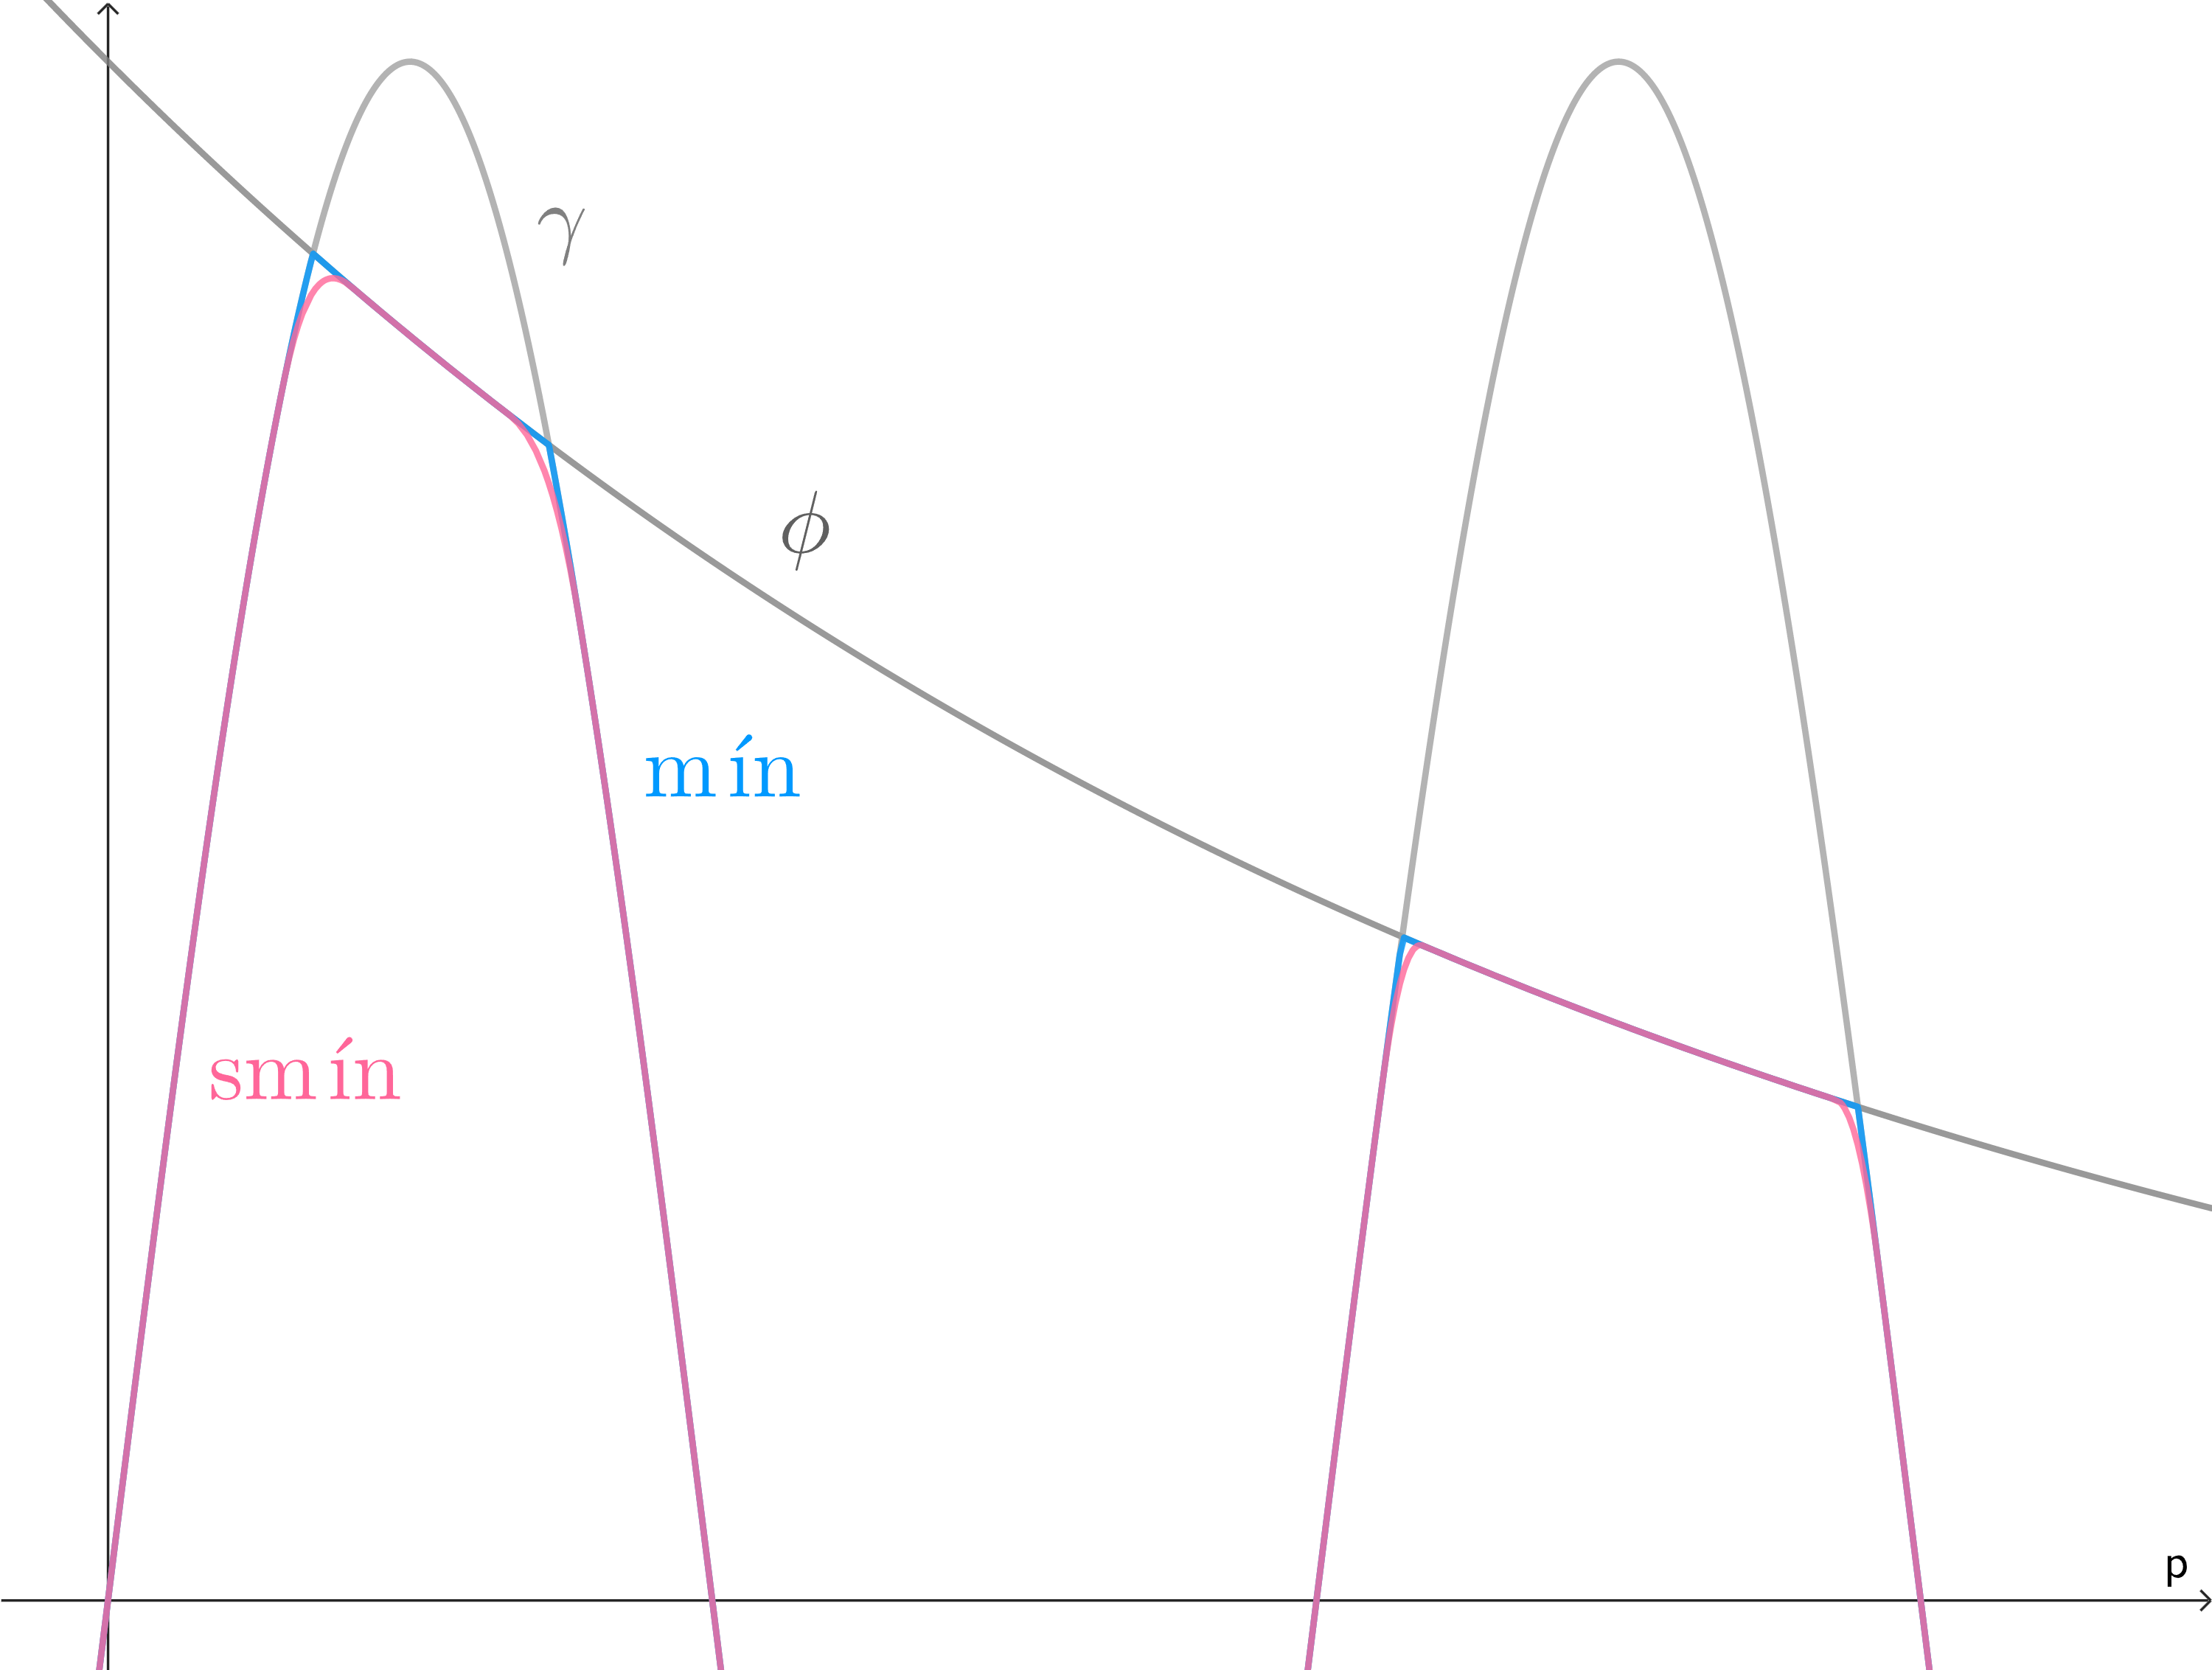
\includegraphics[width=0.95\textwidth]{Plantilla-TFG-master/img/smin_3.png}
        \caption{$k=0.1,\ n=2$}
     \end{minipage}
     \begin{minipage}[c]{0.49\linewidth}
        \centering
        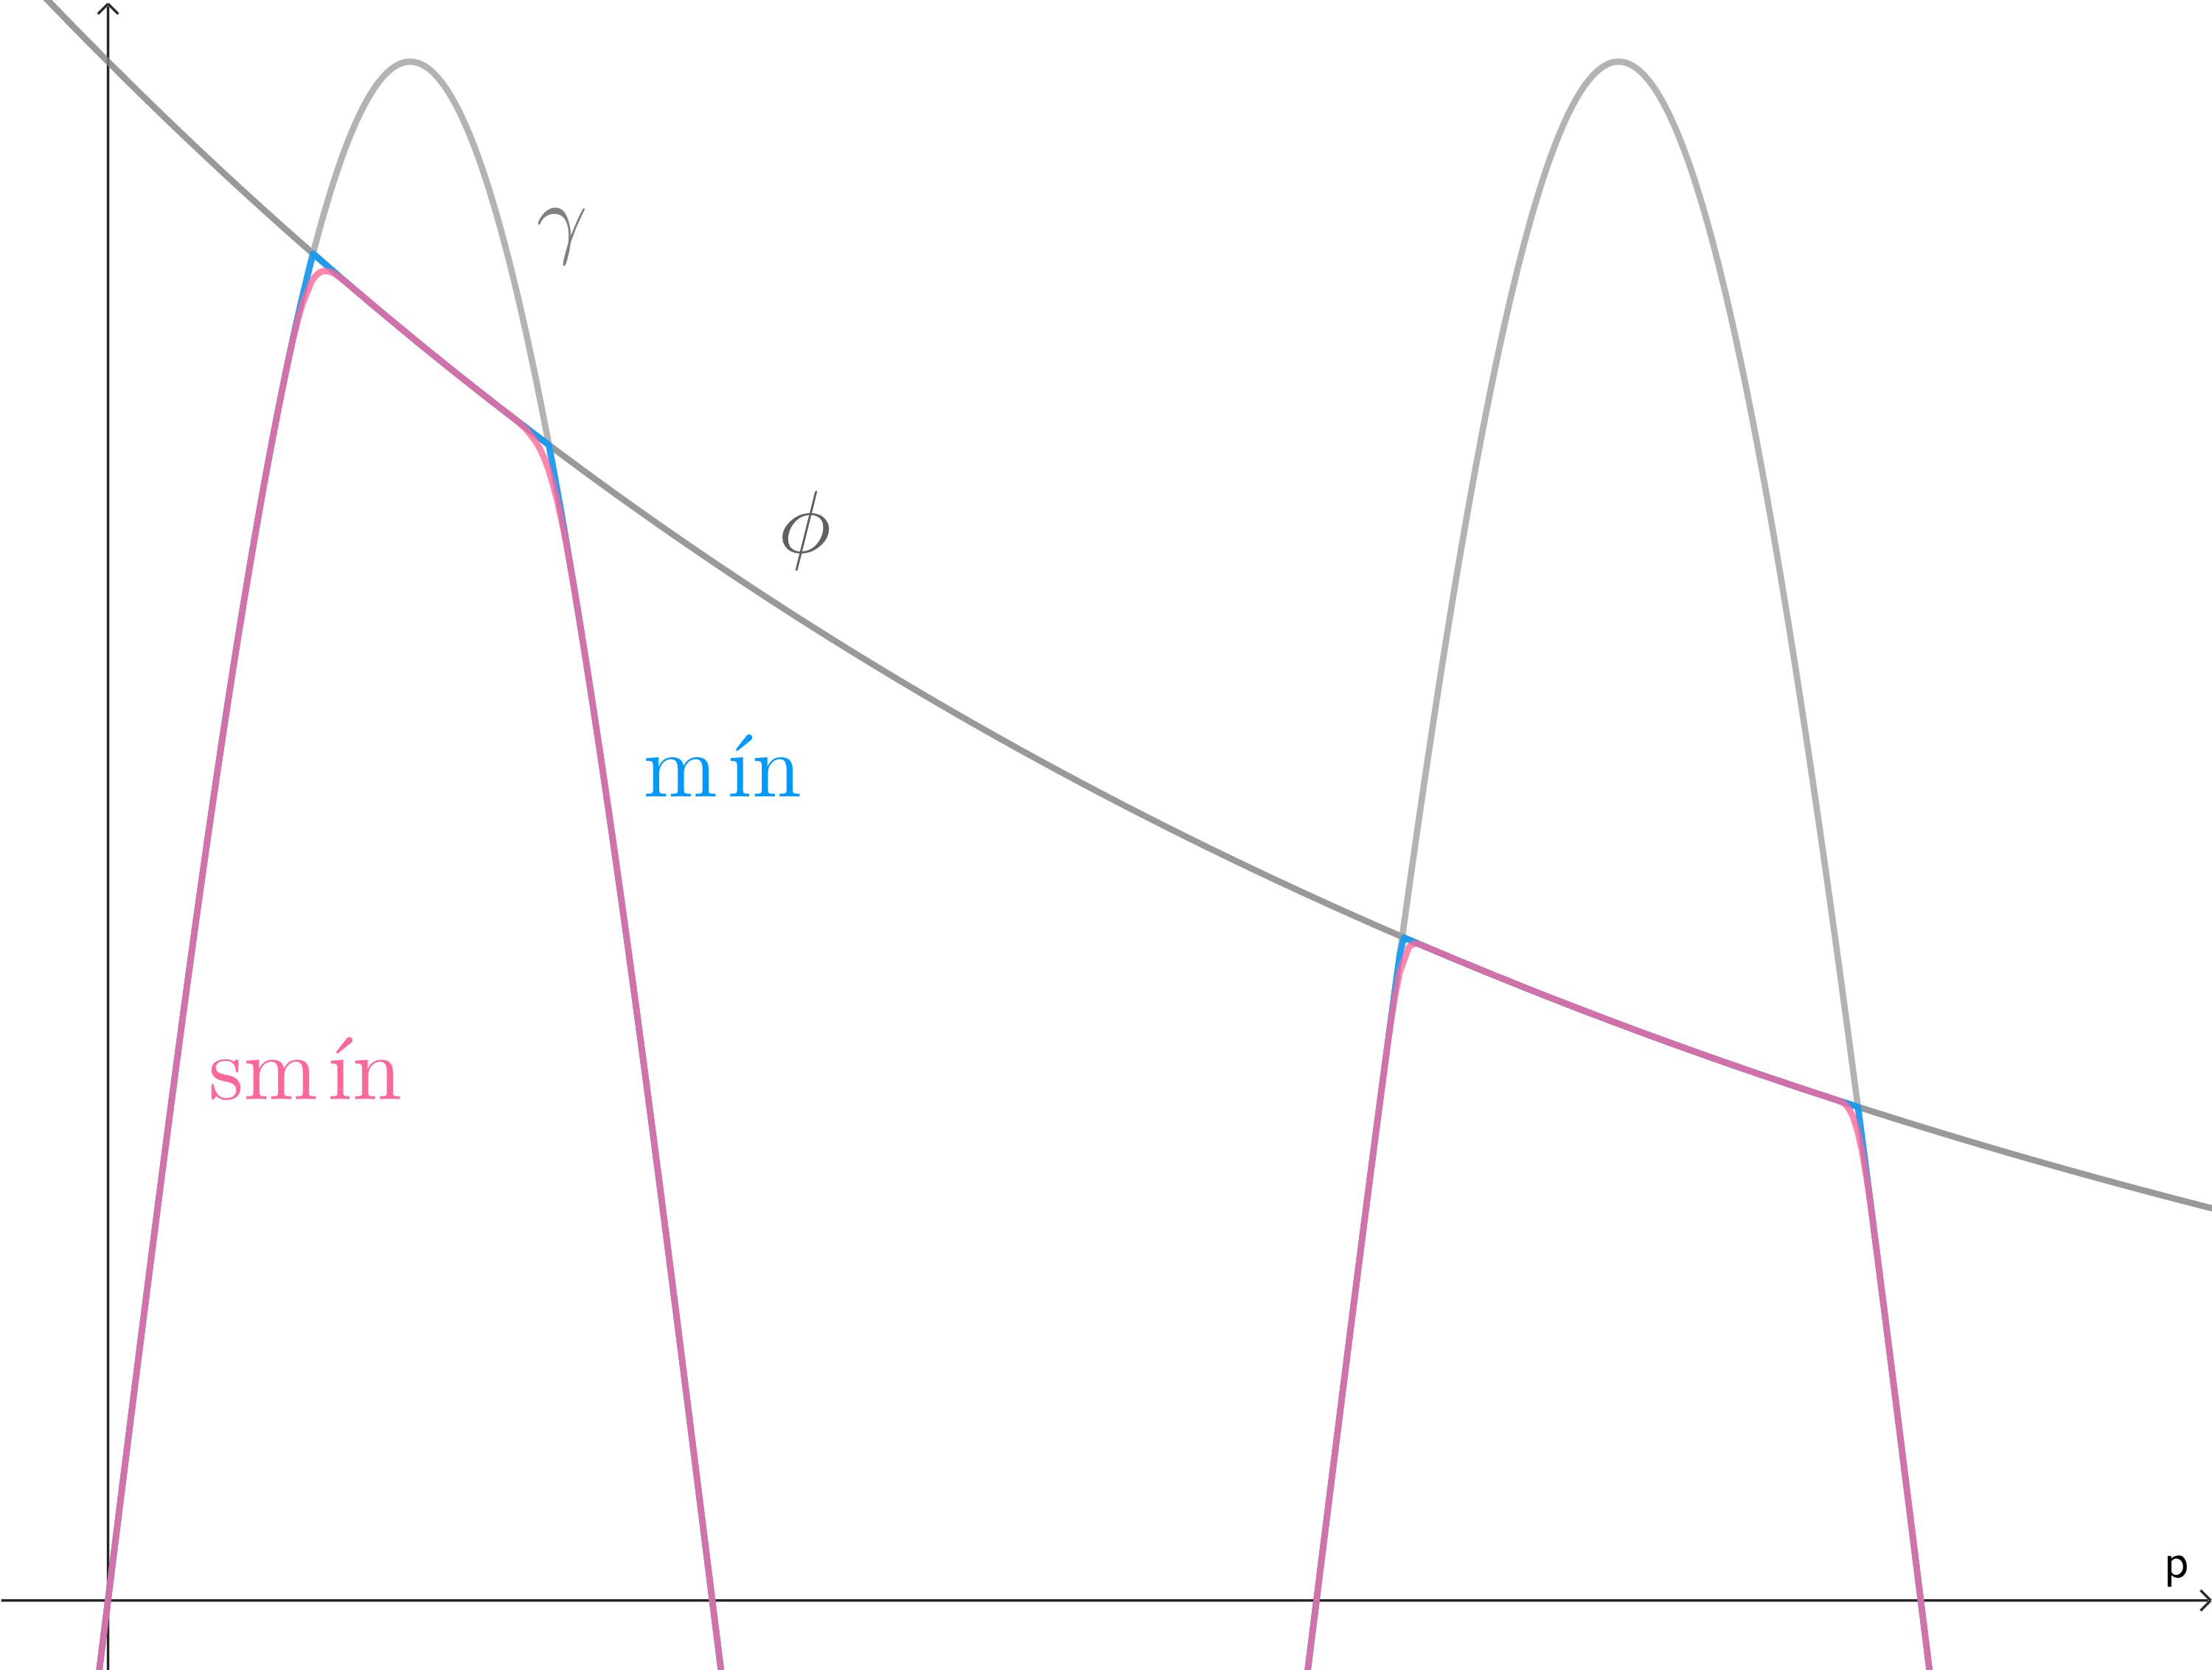
\includegraphics[width=0.95\textwidth]{Plantilla-TFG-master/img/smin_4.png}
        \caption{$k=0.1,\ n=3$}
     \end{minipage}
     \caption{Resultado final de $smin(p)$ }
     \label{fig:smooth2}
\end{figure}





% Por tanto, dadas $\phi$ y $\gamma$, queremos obtener una versión suavizada de $\Min(\phi,\gamma)$ usando interpolación lineal, que llamaremos $\smin$ y tendrá la forma
% \begin{align*}
%           \smin\colon \R^3 &\to \R^3.\\
%           p &\mapsto h(p)\cdot \phi(p) + (1-h(p))\gamma(p) \text{, donde } h \colon \R^3 \to [0,1].
%     \end{align*}


% Pasamos a buscar $h$. Solo queremos modificar la función en los entornos de los puntos en los que intersecan $\phi$ y $\gamma$, de forma que para el resto de puntos debería ser $h=\{0,1\}$. Los puntos de intersección vienen dados como las soluciones de $m(p)=\gamma(p) - \phi(p)$. Podemos además acotar $m(p)$ en el intervalo $[0,1]$ usando $\Min$ y $\Max$, obteniendo un candidato a valor de $h(p)$:
% \begin{equation}
%     \Min\left(\Max\left(\phi(p)-\gamma(p),0\right),1\right) = \Min\left(\Max\left(m(p),0\right),1\right) \in [0,1]
% \end{equation}

% Sin embargo, podemos ver que la interpolación comienza justo en la intersección, mientras que nos gustaría que esto ocurriese antes. Modificamos la expresión anterior para hacer que la intersección sea el punto medio de la interpolación ($h=0.5$):
% \begin{equation}
%    \Min\left(\Max\left(m(p) + \frac{1}{2},0\right),1\right)
% \end{equation}

% Podemos ver los resultados de esta primera aproximación en la \autoref{fig:smooth1}.

% \begin{figure}[!h]
%      \begin{minipage}[c]{0.49\linewidth}
%         \centering
%         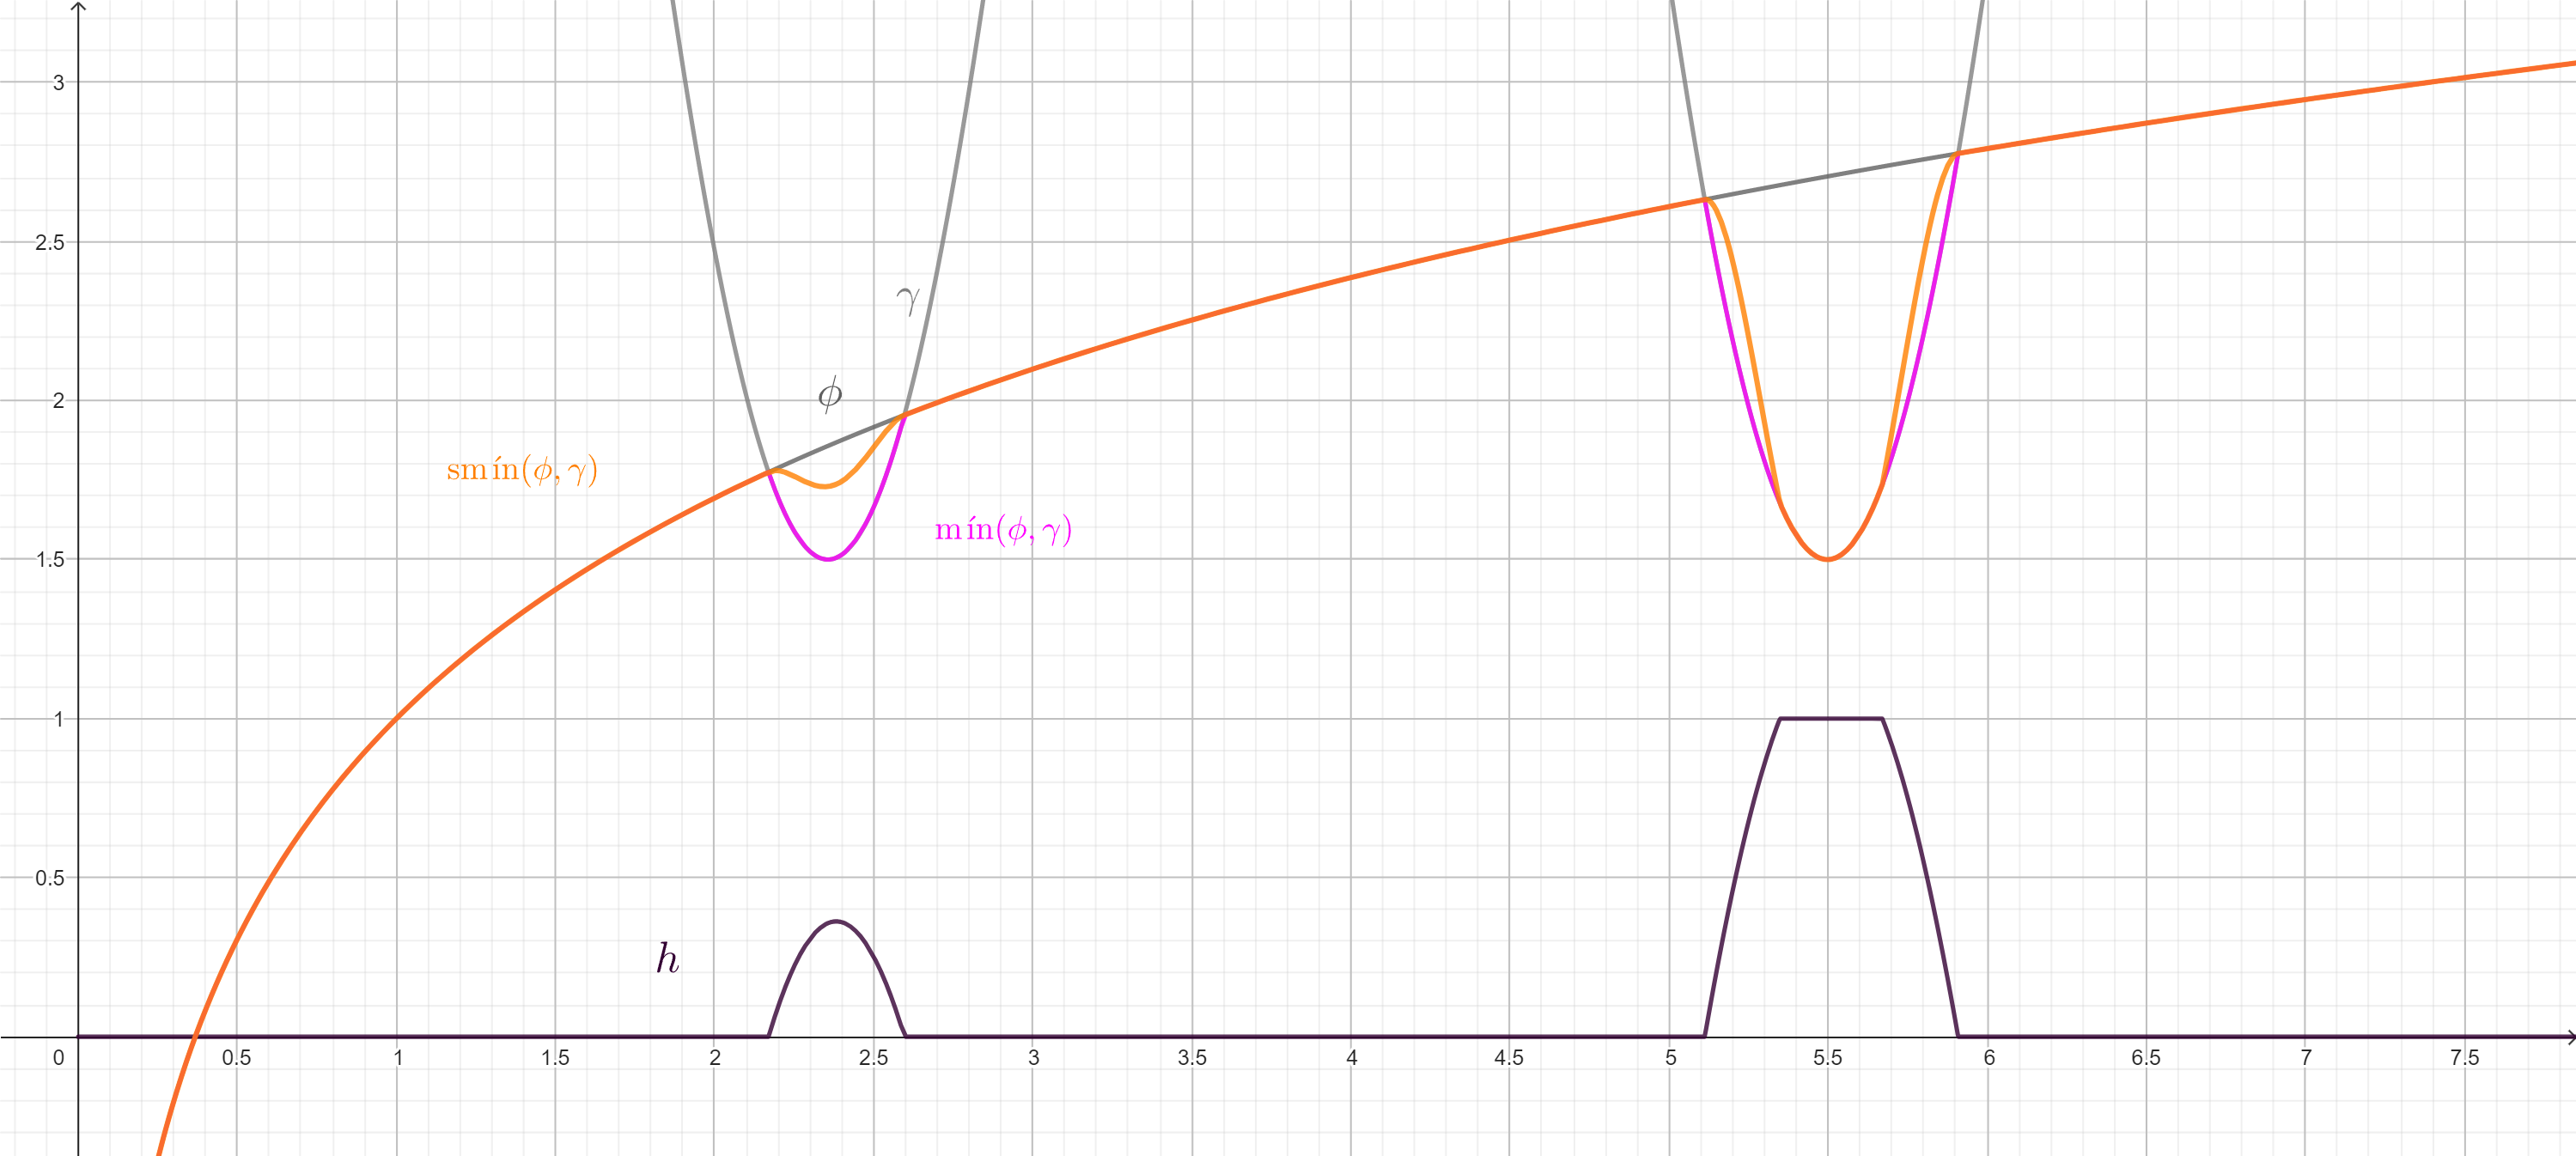
\includegraphics[width=0.95\textwidth]{Plantilla-TFG-master/img/smoothV1_a.png}
%         \caption{$h(p)=0$ en la intersección}
%      \end{minipage}
%      \begin{minipage}[c]{0.49\linewidth}
%         \centering
%         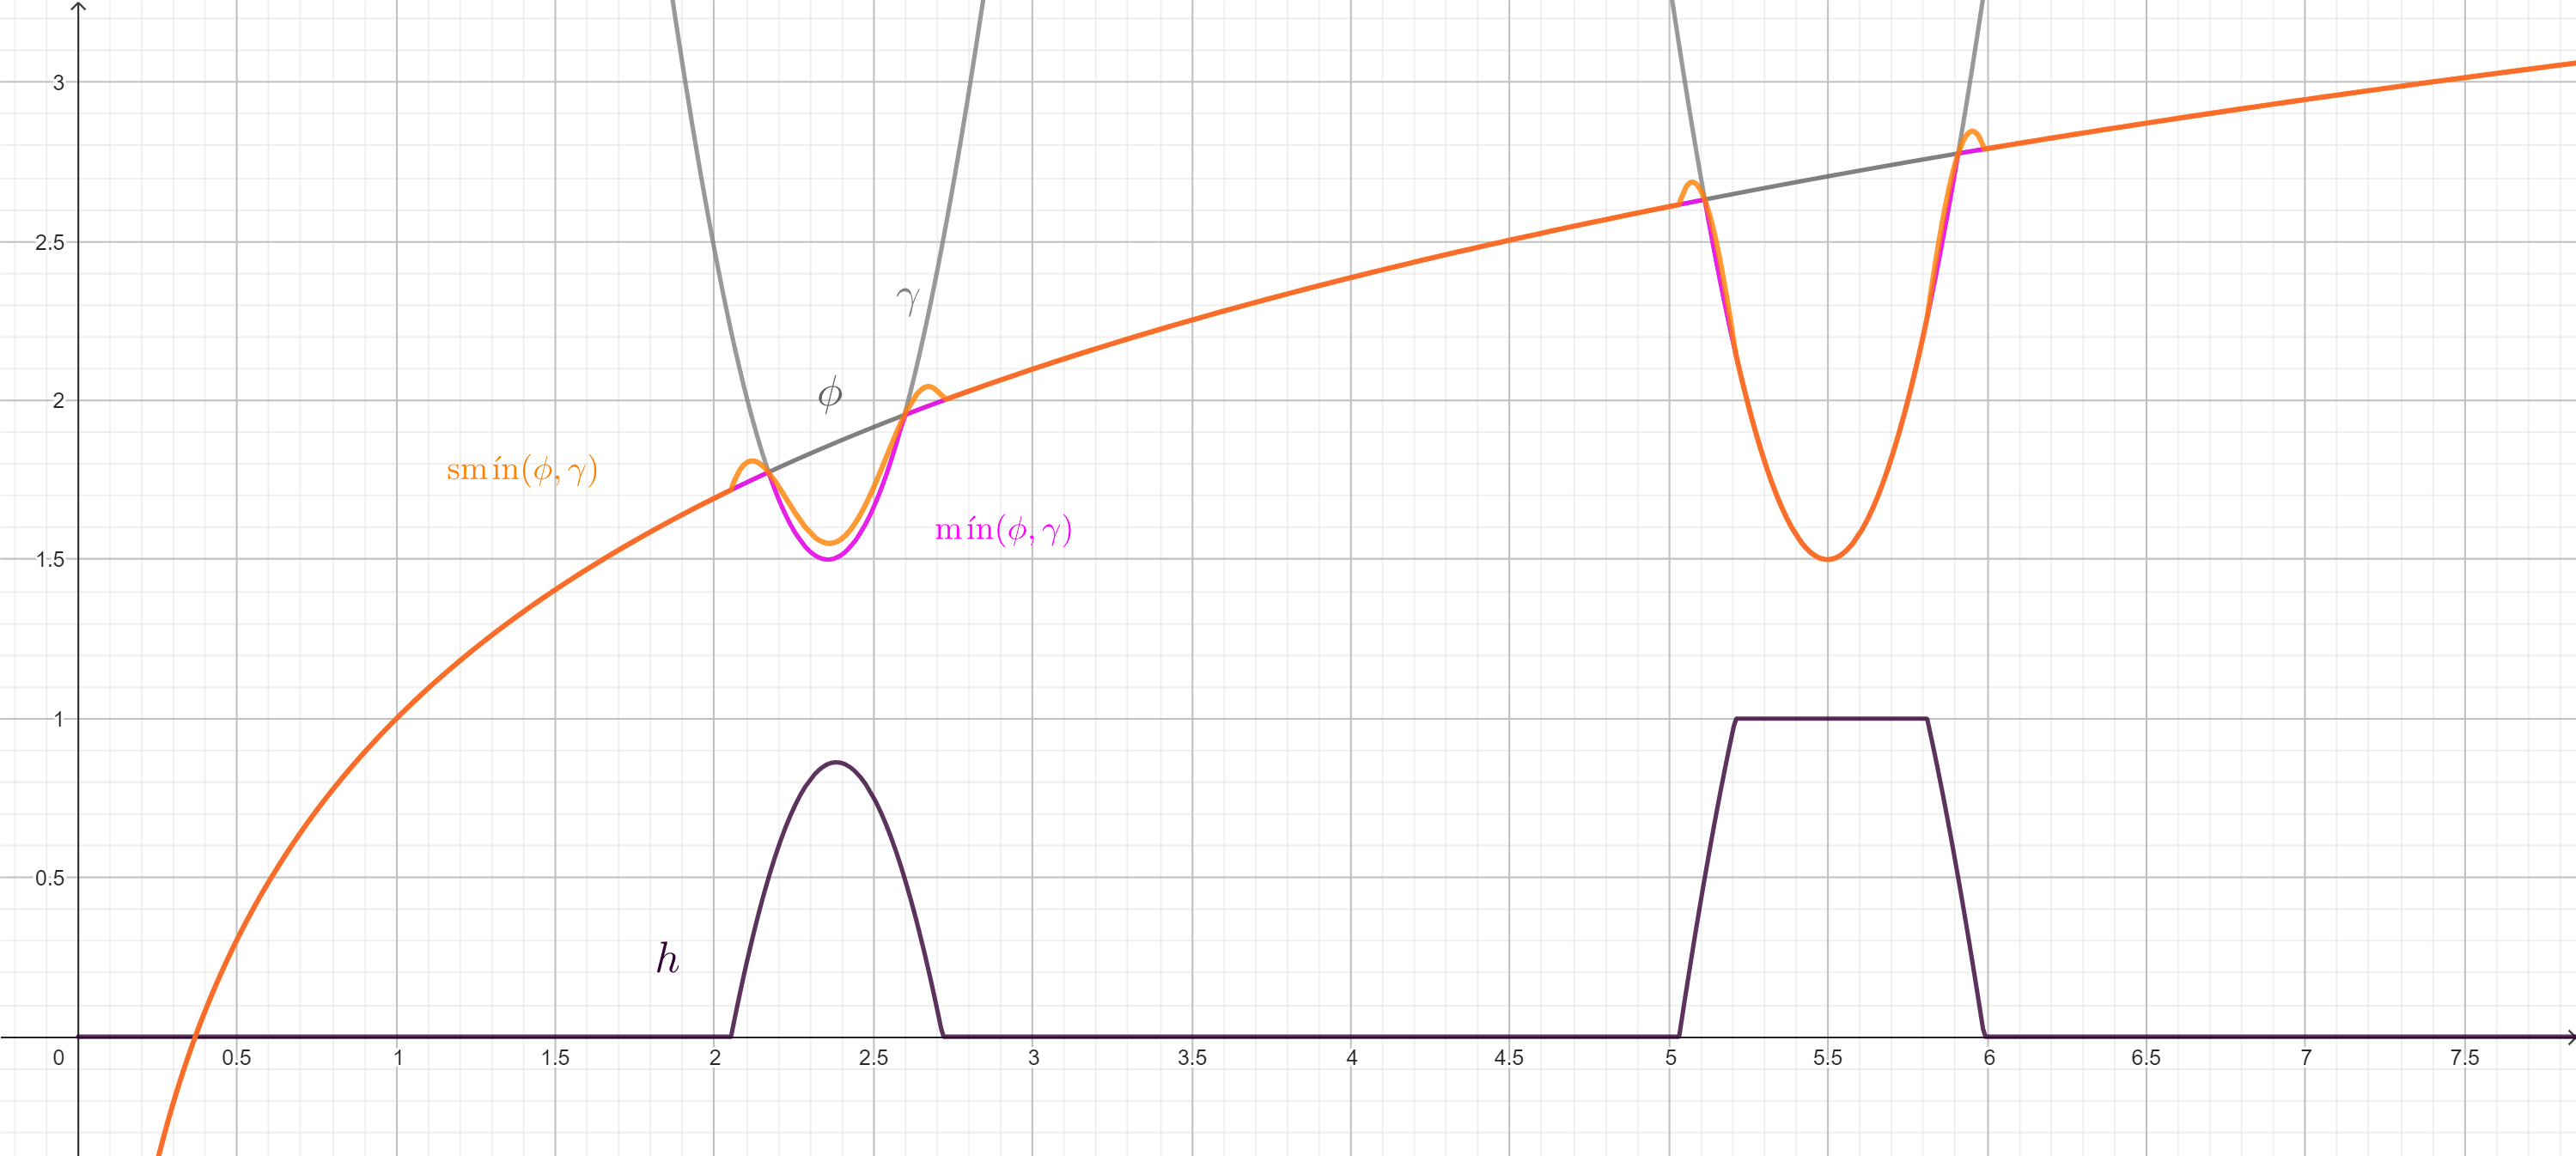
\includegraphics[width=0.95\textwidth]{Plantilla-TFG-master/img/smoothV1_b.png}
%         \caption{$h(p)=0.5$ en la intersección}
%      \end{minipage}
%      \caption{Primera aproximación de la obtención de $h(p)$}
%      \label{fig:smooth1}
% \end{figure}

% Observamos que ahora tenemos un nuevo problema

\begin{definicion}[Operaciones Booleanas Suavizadas]
    Sean $A$ y $B$ isosuperficies generadas por $\phi$ y $\gamma$ respectivamente. La función $\mu$ define la isosuperficie para las siguientes operaciones.
    \begin{itemize}
        \item \textbf{Unión suavizada: } $\mu_{unionS}(p) = \Min(\phi(p),\gamma(p)) - \frac{\Max\left( k - |\phi(p) - \gamma(p)|, 0\right)^n}{2n\cdot k^{n-1}}$.
        \item \textbf{Intersección suavizada: } $\mu_{interS}(p) = -\Min(-\phi(p),-\gamma(p)) + \frac{\Max\left( k - |\phi(p) - \gamma(p)|, 0\right)^n}{2n\cdot k^{n-1}}$.
        \item \textbf{Diferencia suavizada: } $\mu_{difS}(p) = -\Min(-\phi(p),\gamma(p)) + \frac{\Max\left( k - |\phi(p) + \gamma(p)|, 0\right)^n}{2n\cdot k^{n-1}}$.
    \end{itemize}
    La constante $k\in \R^+_0$ controla la influencia del suavizado.        
\end{definicion}

Observamos que los operadores definidos en la \autoref{p:boolean} no son más que un caso particular de estos últimos cuando $k$ tiende a cero. Este método para obtener una versión suavizada de las funciones mínimo y máximo no es el único. Hemos elegido debido a que las funciones obtenidas tienen asociado un coste computacional. Además, su deducción es bastante natural y el efecto que tiene el valor $k$ sobre el resultado final es intuitivo para el usuario. En el artículo que hemos mencionado al inicio de la sección, Íñigo Quílez \cite{article:smooth} presenta otras tres alternativas a esta versión, a la cual él se refiere como \qq{mínimo suavizado polinomial}, y que también son compatibles con \textit{raymarching}.
\begin{itemize}
    \item \textbf{Mínimo suavizado exponencial:} $\smin_{\phi,\gamma}(p) = \frac{-\log_2\left( 2^{-k\phi(p)} + 2^{-k\gamma(p)} ) \right)}{k}$.
    \item \textbf{Mínimo suavizado potencial:} $\smin_{\phi,\gamma}(p) = \left(\frac{\phi(p)^k \cdot \gamma(p)^k}{\phi(p)^k + \gamma(p)^k}\right)^{1/k}$.
    \item \textbf{Mínimo suavizado por raíz:} $\smin_{\phi,\gamma}(p) = \frac{\phi(p) + \gamma(p) - \sqrt{(\phi(p)-\gamma(p))^2+k}}{2}$.
\end{itemize}

La principal ventaja de la versión polinomial respecto a estas es que es la más rápida al ser sus cálculos computacionalmente más baratos. Por otro lado tanto la exponencial como la potencial permiten ser adaptadas fácilmente para calcular el mínimo de un conjunto arbitrario de puntos, útil cuando se trabaja con patrones de voronoi o nubes de puntos. Además, la versión exponencial produce siempre el mismo resultado independientemente del orden en el que se aplique. Es decir,
\begin{equation*}
    \smin_{a,\smin_{b,c}} = \smin_{b,\smin_{a,c}}.
\end{equation*}

En la \autoref{fig:smoothVS} podemos ver un ejemplo de uso de estas versiones, en las que además se ha usado el valor de $w_k$ de la ecuación \autoref{eq:correccion} para interpolar la componente difusa de ambas primitivas usando el método \texttt{mix} de GLSL. Como vemos, no hay diferencias notables entre las distintas versiones, así que nos quedaremos con el método más eficiente: el polinómico.
\begin{figure}[htbp]
    \centering
    \begin{subfigure}[b]{0.25\textwidth}
        \centering
        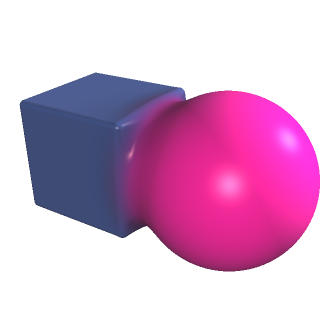
\includegraphics[width=\textwidth]{Plantilla-TFG-master/img/unionMethodOG.png}
        \caption{Polinomial, $k=1.5$}
    \end{subfigure}
    \hfill
    \begin{subfigure}[b]{0.25\textwidth}
        \centering
        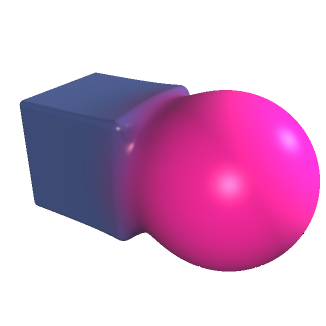
\includegraphics[width=\textwidth]{Plantilla-TFG-master/img/unionMethodExp.png}
        \caption{Exponencial, $k=2.5$}
    \end{subfigure}
    \hfill
    \begin{subfigure}[b]{0.25\textwidth}
        \centering
        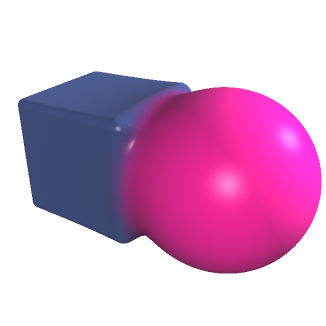
\includegraphics[width=\textwidth]{Plantilla-TFG-master/img/unionMethodRoot.png}
        \caption{Raíz, $k=1$}
    \end{subfigure}
    
    \caption{Diferentes versiones de la unión suavizada}
    \label{fig:smoothVS}
\end{figure}

\subsection{Operaciones afines}
Pasamos ahora a estudiar otro tipo de operaciones que nos permitirán aplicar movimientos rígidos y cambios de escala a las primitivas en la escena. A diferencia de los operadores booleanos, que eran binarios, estas operaciones se aplican a una única primitiva. Su funcionamiento se basará en aplicar una transformación $t:\R^3\to \R^3$ a cada punto de la isosuperficie $S_{\phi}$ para obtener la transformada $S_{\gamma}$. Si queremos saber si un punto $q\in\R^3$ está en $S_{\gamma}$, tenemos que comprobar si su preimagen por la transformación pertenece a $S_{\phi}$. Por tanto, bastará evaluar la SDF original en $t^{-1}(p)$:
\begin{equation*}
    \gamma(p) = \phi(t^{-1}(p)).
\end{equation*}

Este razonamiento funciona bien para transformaciones como las traslaciones o rotaciones, que son movimientos rígidos y mantienen las distancias. Sin embargo, este no es el caso del escalado, ya que si tomamos $l(p) = sp$ con $s\in \R^+_0$
\begin{equation*}
    \Vert p-p'\Vert = d, \text{ luego }  \Vert l(p)-l(p')\Vert = \Vert sp-sp'\Vert = s\Vert p-p'\Vert = s\cdot d,\  \text{ donde } p,p' \in S_{\phi}.
\end{equation*}
Como las distancias se escalan, deberemos hacer lo propio con la función que genere la nueva isosuperficie, aplicándole el mismo factor de escalado $s$ como muestra la \autoref{d:afines}.

\begin{definicion}[Operaciones afines]\label{d:afines}
    Sea $A$ una isosuperficie. Definimos las SDFs para las siguientes operaciones.
    \begin{itemize}
        \item \textbf{Traslación de vector $\boldsymbol{v\in R^3}$: } $\sdf_{traslacion}(p) = \sdf_{A}(p - v)$.
        \item \textbf{Escalado uniforme de dimensiones $\boldsymbol{(s,s,s)\in \R^3}$: } $\sdf_{escalado}(p) = \sdf_{A}(p/s)\cdot s$.
        \item \textbf{Rotaciones de ángulo $\boldsymbol{\alpha\in \R}$ sobre los ejes $\boldsymbol{x,y,z}$: }
        \begin{align*}
            \sdf_{rotX}(p) &= \mu_{A}(R_x^{-1}(\alpha)\cdot p^t),\ \text{donde } R_x(\alpha) = 
            \begin{pmatrix}
                1&0&0\\
                0&\cos(\alpha) & -\sin(\alpha) \\
                0&\sin(\alpha) & \cos(\alpha) 
                \end{pmatrix},\\[10pt] 
            \sdf_{rotY}(p) &= \mu_{A}(R_y^{-1}(\alpha)\cdot p^t),\ \text{donde } R_y(\alpha) = \begin{pmatrix}
            \cos(\alpha) &0& \sin(\alpha)\\
            0&1&0\\
            -\sin(\alpha) &0& \cos(\alpha) 
            \end{pmatrix},\\[10pt]
            \sdf_{rotZ}(p) &= \mu_{A}(R_z^{-1}(\alpha)\cdot p^t),\ \text{donde } R_z(\alpha) = \begin{pmatrix}
            \cos(\alpha) & -\sin(\alpha) & 0\\
            \sin(\alpha) & \cos(\alpha) & 0\\
            0&0&1
            \end{pmatrix}.
        \end{align*}
    \end{itemize}
\end{definicion}

Observamos que en este caso sí que obtenemos funciones distancia con signo como resultado, al contrario de lo que ocurría con las operaciones booleanas.
\begin{figure}[ht!]
    \centering
    \begin{subfigure}[b]{0.24\textwidth}
        \centering
        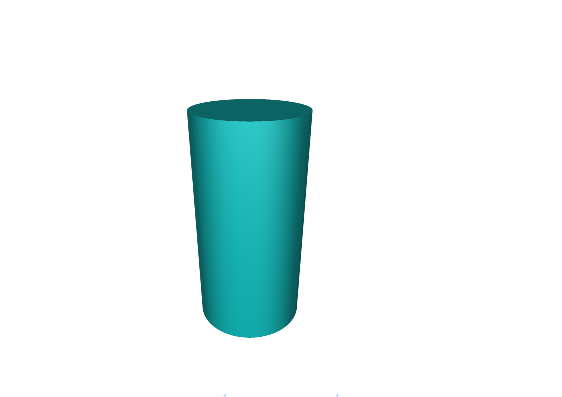
\includegraphics[width=\textwidth]{Plantilla-TFG-master/img/afin_og.png}
        \caption{Original}
    \end{subfigure}
    \hfill
    \begin{subfigure}[b]{0.24\textwidth}
        \centering
        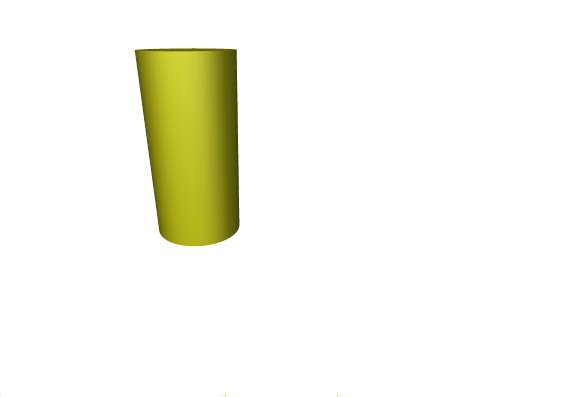
\includegraphics[width=\textwidth]{Plantilla-TFG-master/img/afin_trans.png}
        \caption{Traslación}
    \end{subfigure}
    \hfill
    \begin{subfigure}[b]{0.24\textwidth}
        \centering
        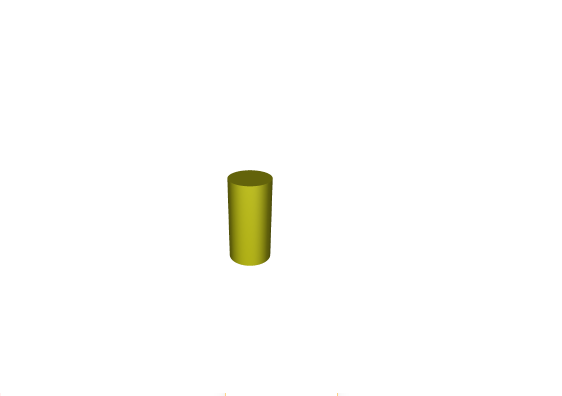
\includegraphics[width=\textwidth]{Plantilla-TFG-master/img/afin_scale.png}
        \caption{Escalado uniforme}
    \end{subfigure}
    \hfill
    \begin{subfigure}[b]{0.24\textwidth}
        \centering
        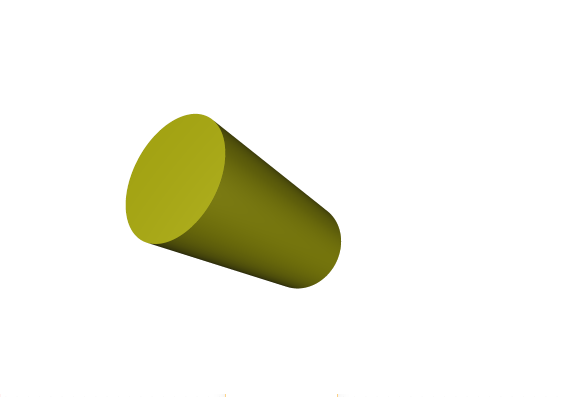
\includegraphics[width=\textwidth]{Plantilla-TFG-master/img/afin_rot.png}
        \caption{Rotación}
    \end{subfigure}
    \hfill
   
    \caption{Ejemplos de uso de los operadores afines}
\end{figure}

\subsection{Operaciones deformantes}
Siguiendo el mismo razonamiento, podemos definir operaciones que modifiquen la geometría de la superficie aplicando rotaciones o traslaciones al punto en el que se evalúa la función distancia con signo original. De esta forma podemos obtener operadores que de otra forma sería mucho más complicado implementar, como la torsión o el redondeo de los bordes de una primitiva \cite{deform}.

\begin{definicion}[Operaciones Deformantes]
    Sea $A$ una isosuperficie. La función $\mu$ define la isosuperficie para las siguientes operaciones.
    \begin{itemize}
        
        \item \textbf{Torsión: } $\mu_{torsion}(p) = \sdf_{A}(p')$, con $p' = R_z(ky)\cdot (x,z,y)^t$.
        \item \textbf{Plegado: } $\mu_{plegado} =\sdf_{A}(p')$, con $p' = R_z(kx)\cdot p^t$.
        \item \textbf{Redondeo: } $\mu_{redondeo}(p) = \sdf_{A}(p) - k$.
        \item \textbf{Desplazamiento: } $\mu_{desplazamiento}(p) = \sdf_{A}(\delta(p))$.
        \item \textbf{Elongación de tamaño $\boldsymbol{h\in \R^3}$: } $\sdf_{elongacion}(p) = \mu_{A}(p')$, con $p' = p - c(p, -h, h)$.
    \end{itemize}
    En estas definiciones,
    \begin{itemize}
        \item $k\in \R^+_0$ controla la intensidad de la deformación,
        \item $\delta\colon \R^3\to \R^3$ es un patrón de desplazamiento,
        \item $R_z(\alpha)\in \mathcal{M}_3(\R)$ es la matriz de rotación de ángulo $\alpha$ sobre el eje $z$ dada en la \autoref{d:afines},
        \item $c\colon \R^3\times \R^3 \times \R^3 \to \R^3,\ c(x,a,b)$ acota cada componente de $x$ entre las de $a$ y $b$.
    \end{itemize}
\end{definicion}

Las únicas operaciones que nos proporcionan una función distancia con signo como resultado son el redondeo y la elongación. El resto es recomendable usarlas lo menos posible, pues las isosuperficies que generan pueden presentar fallos al ser renderizadas.
\begin{figure}[ht!]
    \centering
    \begin{subfigure}[b]{0.30\textwidth}
        \centering
        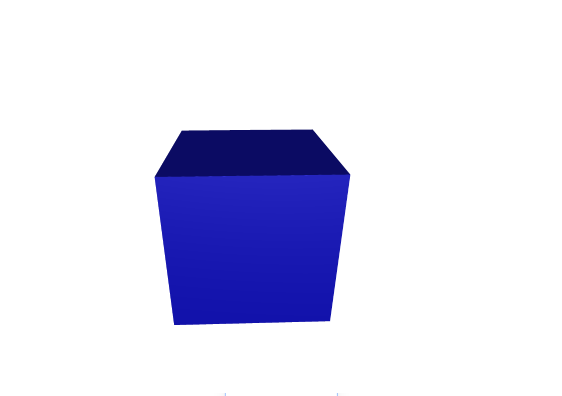
\includegraphics[width=\textwidth]{Plantilla-TFG-master/img/deform_og.png}
        \caption{Original}
    \end{subfigure}
    \hfill
    \begin{subfigure}[b]{0.30\textwidth}
        \centering
        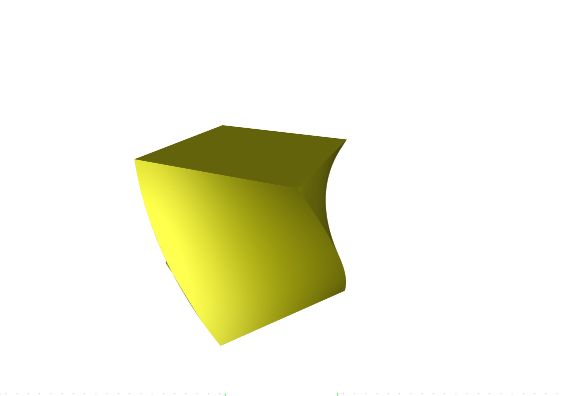
\includegraphics[width=\textwidth]{Plantilla-TFG-master/img/deform_twist.png}
        \caption{Torsión}
    \end{subfigure}
    \hfill
    \begin{subfigure}[b]{0.30\textwidth}
        \centering
        
\includegraphics[width=\textwidth]{Plantilla-TFG-master/img/deform_bend.png}
        \caption{Plegado}
    \end{subfigure}
    \hfill
    \begin{subfigure}[b]{0.30\textwidth}
        \centering
        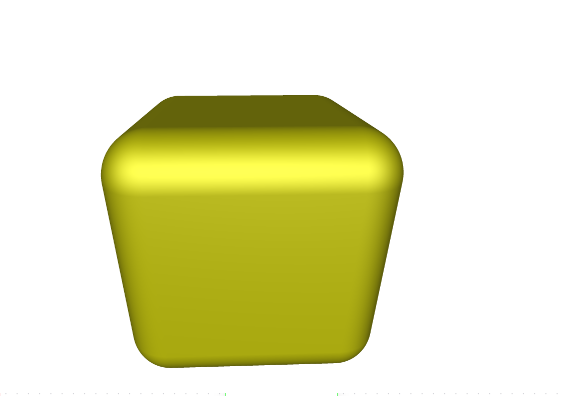
\includegraphics[width=\textwidth]{Plantilla-TFG-master/img/deform_round.png}
        \caption{Redondeo}
    \end{subfigure}
    \hfill
    \begin{subfigure}[b]{0.30\textwidth}
        \centering
        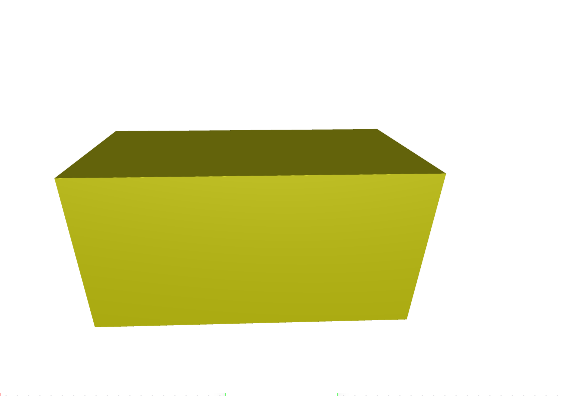
\includegraphics[width=\textwidth]{Plantilla-TFG-master/img/deform_elong.png}
        \caption{Elongación}
    \end{subfigure}
    
    \caption{Ejemplos de uso de los operadores de deformación}
\end{figure}

\subsection{Operaciones de repetición}
También podemos usar la técnica de cambiar el punto en el que evaluamos la función distancia para, en lugar de modificar la geometría original, añadir copias de la primitiva identificando varios puntos con uno que pertenezca a la isosuperficie. La manera más inmediata de conseguir esto es a través de la función valor absoluto, que nos permitirá identificar la componente de cada punto con su opuesta para generar simetrías, y el operador módulo, que identificará puntos a una distancia fija en cada eje.

\begin{definicion}[Operadores de Posicionamiento]\label{d:posicionamiento}
    Sea $A$ una isosuperficie. La función $\mu$ define la isosuperficie para las siguientes operaciones.
    \begin{itemize}
        \item \textbf{Simetrías sobre los ejes $\boldsymbol{x,y,z}$:}
        \begin{gather*}
            \mu_{simX}(p) = \sdf_{A}(\vert x\vert, y, z),\quad \mu_{simY}(p) = \sdf_{A}(x, \vert y\vert,  z),\\[5pt] \mu_{simZ}(p) = \sdf_{A}(x,y,\vert z\vert).
        \end{gather*}
        \item \textbf{Simetrías sobre los planos $\boldsymbol{xy,xz,yz}$:}
        \begin{gather*}
            \mu_{simXY}(p) = \sdf_{A}(\vert x\vert, \vert y\vert, z),\quad \mu_{simXZ}(p) = \sdf_{A}(\vert x\vert, y,  \vert z\vert),\\[5pt]\mu_{simYZ}(p) = \sdf_{A}(x,\vert y\vert ,\vert z\vert).
        \end{gather*}
        \item \textbf{Repetición $\boldsymbol{l\in \N^3}$ veces en los ejes $\boldsymbol{x,y,z}$ con separación $\boldsymbol{s\in\R}$:} 
        \begin{equation*}
            \mu_{rep}(p) = \sdf_{A}(p - s\cdot c\left(r\left(\frac{p}{s}\right), -l, l\right).
        \end{equation*}
        \item \textbf{Repetición infinita:}
        \begin{equation*}
            \mu_{repInf}(p) = \sdf_{A}\left((p+\frac{l}{2}\mod l )- \frac{l}{2}\right).
        \end{equation*}
    \end{itemize}
    En estas definiciones,
    \begin{itemize}
        \item $c\colon \R\times\R\times\R\to \R,\ c(x,a,b) = \Min(\Max(x, a), b)$ acota $x$ en $[a,b]$,
        \item $r\colon \R^3 \to \R^3$ redondea las componentes de un vector a sus enteros más cercanos.
    \end{itemize}
\end{definicion}
\begin{figure}[ht!]
    \centering
    \begin{subfigure}[b]{0.48\textwidth}
        \centering
        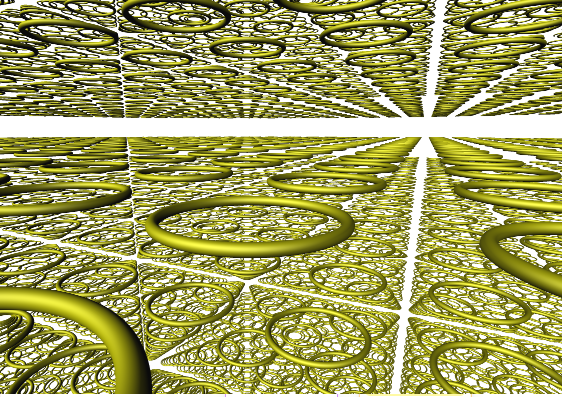
\includegraphics[width=\textwidth]{Plantilla-TFG-master/img/rep.png}
        \caption{Repetición infinita}
    \end{subfigure}
    \hfill
    \begin{subfigure}[b]{0.48\textwidth}
        \centering
        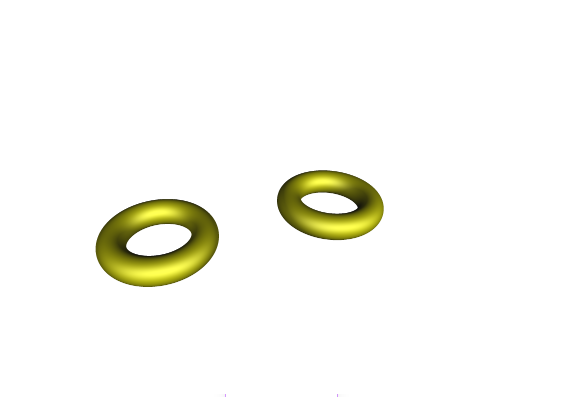
\includegraphics[width=\textwidth]{Plantilla-TFG-master/img/sym.png}
        \caption{Simetría}
    \end{subfigure}
    \hfill
        
    \caption{Ejemplos de uso de los operadores de repetición}
\end{figure}

Las funciones obtenidas no son en general funciones distancia con signo. Esto ocurre en los siguientes casos.
\begin{itemize}
    \item Al aplicar simetrías, cuando el objeto interseca el plano de simetría.
    \item En el caso de la repetición infinita, cuando las dimensiones del objeto sean mayores o iguales a $l/2$.
    \item Siempre para la repetición finita, como consecuencia de usar la función máximo. 
\end{itemize}

No obstante, este tipo de operaciones evidencia el potencial que tienen las funciones distancia con signo en cuanto a eficiencia a la hora de generar nuevas superficies, ya que podemos visualizar miles de objetos al precio de uno. Por ejemplo, podríamos generar un campo de césped a partir de una única brizna de hierba, o modelar solo una fracción de un objeto y generar el resto usando simetrías.



\section{Obtención de una SDF a partir de ecuaciones implícitas}\label{sec:aprox}
Empezábamos el capítulo diciendo que una de las representaciones más comunes de una superficie es a través de implícitas, pero hasta ahora nos hemos centrado en estudiar un subconjunto de esta familia. Si intentásemos aplicar el algoritmo de \textit{raymarching} a una función implícita cualquiera podríamos observar que el resultado presenta defectos, tales como deformaciones o grietas, o que incluso no se visualiza. Veamos qué podemos hacer para, dada una función implícita $\phi$ cualquiera, obtener información aproximada de $S_\phi$ \cite{article:aprox}. Esto nos será útil cuando no conozcamos o no podamos calcular explícitamente la función distancia con signo de una superficie, pero sí su ecuación implícita.

\begin{proposicion}
    Sea $\phi\colon \R^3\to\R$ una función implícita cualquiera. Entonces
    \begin{equation*}    
        \vert \sdf_{S_\phi}(p)\vert \le \frac{\vert \phi(p)\vert}{\Vert \nabla\phi(p)\Vert}.
    \end{equation*}
\end{proposicion}
\begin{proof}
    Fijamos el punto $p$ del cual queremos aproximar la distancia a $S_{\phi}$. Sea $q$ el punto de $S_\phi$ más cercano a $p$ y $v=\vec{pq}$. Queremos calcular la distancia de $p$ a $S_\phi$, que será justamente $\Vert v\Vert$. Asumiendo que $\phi$ es diferenciable en $p$, podemos realizar el desarrollo de Taylor de $\phi$ centrado en $p$:
    \begin{equation*}
        \phi(p) = \phi(p) + \nabla(p)\cdot (p+v -p) + \mathcal{O}(\vert p+v-p)\vert^2) = \phi(p) + \nabla(p)\cdot v + \mathcal{O}(\vert v\vert^2).
    \end{equation*}

    Suponemos ahora que $p$ está cerca de $S_\phi$, luego existe un $\varepsilon>0$ tal que  $\vert v\vert < \varepsilon$, y podemos obviar el residuo y $\phi(p)\approx \phi(q) = \phi(p+v)$. Como $\phi(q)=0$, tenemos que
    \begin{equation*}
        0 = \vert \phi(p+v)\vert \le \vert \phi(p) + \nabla(p)\cdot v \vert \le \vert \phi(p)\vert - \vert \nabla(p)\cdot v \vert         \le \vert \phi(p)\vert - \Vert \nabla(p)\Vert\cdot \Vert v \Vert,
    \end{equation*}
    donde hemos usado la desigualdad triangular y la linealidad del producto escalar. De esta expresión, finalmente deducimos que
    \begin{equation*}
        \Vert v\Vert \le \frac{\vert \phi(p)\vert}{\Vert \nabla(p)\Vert}.\qedhere
    \end{equation*}
\end{proof}
\begin{corolario}
    Sea $\phi\colon \R^3\to \R$ lipschitziana con constante $L$. Entonces
    \begin{equation*}    
        \vert \sdf_{S_\phi}(p)\vert \le \frac{\vert \phi(p)\vert}{\vert L\vert}.
    \end{equation*}
\end{corolario}

Este resultado solo nos proporciona una cota superior de la función distancia (sin signo). En nuestro caso esto es suficiente, pues esta nos sigue permitiendo representar la frontera de $S_{\phi}$. En su artículo \cite{art:impSdf}, Pierre-Alain Fayolle describe un método para obtener un SDF asociado a una superficie implícita que representa de manera exacta su frontera. Para ello descompone el SDF como 
\begin{equation*}
    sdf_{S_{\phi}}(p;\theta) = \phi(p)g(p;\theta)\quad \text{ o }\quad sdf_{S_{\phi}}(p;\theta) = sign(\phi(p))g(p;\theta),
\end{equation*}

donde $g$ es una función paramétrica de parámetros $\theta$ y $sign$ es una versión suavizada de la función signo, por ejemplo $sign(x) = \tanh{(kx)}$ con $k\in\R$. Para obtener la expresión de $g$ introduce la función implícita $\phi$ en la capa final de una red neuronal entrenada para  minimizar una función pérdida asociada al SDF, y para ajustar $\theta$ expresa $sdf_{S_{\phi}}(p;\theta)$ como la solución de un problema variacional. No obstante, esta técnica está fuera del ámbito de este trabajo, de forma que nos limitaremos a obtener la cota de la función distancia.

\section{Implicitación de parametrizaciones racionales con bases de Gröbner}

Ahora que sabemos representar las superficies generadas por una ecuación implícita cualquiera, nos proponemos ser capaces de representar también superficies definidas paramétricamente. Para ello fijaremos un anillo conmutativo $A$ y un conjunto de variables distintas $X=\{x_1,\dots, x_n\}$. Nuestro objetivo será, dado un conjunto $V\subseteq A^n$ por las ecuaciones paramétricas
\begin{align*}
    x_1 &= g_1(t_1,\dots, t_r),\\
    &\vdots \\
    x_n &= g_n(t_1,\dots, t_r),
\end{align*}
donde $g_i$ son polinomios de varias variables en $A$, obtener una ecuación implícita para $V$. En el caso que nos atañe $A=\R^3$, pero presentaremos todos los resultados de forma general.\newline

El contenido de esta sección está fuertemente basado en el libro Ideals, Varieties, and Algorithms de Cox, Little y O'Shea \cite{ideals_varieties}, el cual introduce de forma bastante completa resultados y algoritmos de álgebra conmutativa. Empezaremos explicando a qué nos referimos con polinomios de varias variables y recordando el concepto de ideal y sus propiedades. Después veremos que este problema equivale a uno de pertenencia a un ideal y cómo resolverlo usando la teoría de bases de Groebner.

\subsection{Polinomios en varias variables}
Estamos acostumbrados a trabajar con polinomios de una única variable como una suma o colección de monomios. Podemos mantener esta filosofía en el caso de varias variables adaptando el concepto que tenemos de estos.

\begin{definicion}
    Llamamos \textbf{monomio} en $X$ al producto de la forma
    $$x_1^{\alpha_1} \cdots x_n^{\alpha_n}\quad,\ \alpha_i \in \N,\ i\in\{1,\dots, n\}.$$
    Lo denotaremos como $X^{\alpha}$, y diremos que $\alpha\in \N^n$ es el \textbf{exponente} del monomio.
\end{definicion}

\begin{definicion}
    Definimos el \textbf{polinomio} $f:A^n\to A$ en $X$ con coeficientes en $A$ a toda combinación lineal finita de monomios
    \begin{align*}
        f = \sum_{\alpha\in \N^n} a_{\alpha} X^{\alpha}.
    \end{align*}

\end{definicion}

\begin{proposicion}
    El conjunto de polinomios es un anillo conmutativo. En concreto, para
     $$ f = \sum_{\alpha\in \N^n} a_{\alpha} X^{\alpha}\quad \text{ y }\quad g = \sum_{\beta\in \N^n} a_{\beta} X^{\beta},$$ 
     las operaciones internas del anillo son las siguientes.
    \begin{itemize}
        \item Suma heredada de $A$: $(f+g)(a) = f(a) + g(a)$.
        \item Producto de convolución: $(fg)(a) = \sum_{\alpha} \sum_{\beta+\gamma=\alpha} f(a)g(a)$.
    \end{itemize}
    Denotaremos como  $A[X] = A[x_1,\dots, x_n]$ a este anillo.
\end{proposicion}

En las siguientes secciones veremos que el problema de pertenencia de polinomios a un ideal se puede resolver mediante el procedimiento de la división. Este es bien conocido en polinomios de una variable, y ahora queremos extenderlo a un número arbitrario de ellas y varios divisores. Para ello en primer lugar necesitaremos una forma de ordenar los monomios que forman un polinomio. En una variable la forma \qq{natural} de comparar dos monomios es a través de su exponente. En el caso de varias variables la elección no es tan clara, y hay varias opciones que parecen igual de válidas. Vamos a formalizar el concepto de orden para introducir algunas de las posibilidades de las que disponemos. 

\begin{definicion}
    Un \textbf{orden total} sobre un conjunto $\Delta$ es una relación binaria $\le$ que cumple las siguientes propiedades.
    \begin{enumerate}
        \item Reflexiva: $a\le a,\ \text{para todo } a\in \Delta$.
        \item Transitiva: si $a\le b$ y $b\le c$ entonces $a\le c,\ \text{para todo } a,b,c\in \Delta$.
        \item Antisimétrica: si $a\le b$ y $b\le a$ entonces $a\le b,\ \text{para todo } a,b\in \Delta$.
        \item Completitud: $a\le b$ o $b\le a,\ \text{para todo } a,b\in \Delta$.
    \end{enumerate}
\end{definicion}
\begin{definicion}
    Un \textbf{orden admisible} es un orden total $\le$ sobre $\N^n$ cumpliendo
    \begin{enumerate}
        \item $(0,\dots ,0) \le \alpha,\ \text{para todo } \alpha \in \N^n$,
        \item si $\alpha < \beta$ entonces $\alpha + \gamma < \beta + \gamma,\ \text{para todo } \alpha,\beta,\gamma \in \N^n$.
    \end{enumerate}
\end{definicion}
\begin{proposicion}
    Todo orden admisible es un buen orden, esto es, todo subconjunto no vacío tiene un elemento mínimo.
\end{proposicion}

A partir de ahora siempre supondremos que todo orden que usemos es admisible en $\N^n$, luego podemos ordenar los monomios que conforman un polinomio ordenando sus exponentes según dicho orden. Veamos algunos de los órdenes más usados. 

\begin{definicion}
    Definimos el \textbf{orden lexicográfico} $\le_{\text{lex}}$ como
    \begin{equation*}
        \alpha \lex \beta \iff \begin{cases}
            \alpha  = \beta \\
            \quad\text{ó}   \\
            \alpha_i < \beta_i \text{, donde $i$ es el primer índice tal que } \alpha_i \neq \beta_i.
        \end{cases}
    \end{equation*}
\end{definicion}

% \begin{proof}
%     Es inmediato que es total, ya que $\le$ en $\N$ lo es. Veamos las otras condiciones.
%     \begin{enumerate}
%         \item Tomamos $\alpha \in \N^n$ tal que $\alpha\neq (0,\dots,0)$ y sea $i$ el primer índice tal que $\alpha_i \neq 0$. Entonces $0< \alpha_i$, de donde $(0,\dots, 0) \lex \alpha$.
%         \item Sean $\alpha$ y $\beta$ tales que $\alpha\lex \beta$, e $i$ el primer índice tal que $\alpha_i < \beta_i$
%     \end{enumerate}
% \end{proof}

\begin{definicion}
    Dado $\omega\in \N^n$, un orden admisible $\le$ se dice \textbf{$\boldsymbol{\omega}$-graduado} cuando
    \begin{equation*}
        \alpha\le \beta \text { implica que } \langle \alpha, \omega\rangle  < \langle \beta, \omega\rangle,
    \end{equation*}
    donde $\langle \alpha, \omega\rangle$ se llama el \textbf{$\boldsymbol{w}$-grado} de $\alpha$ y se define como
    \begin{equation}
        \langle \alpha, \omega\rangle = \alpha_1 \omega_1 + \cdots + \alpha_n \omega_n.
    \end{equation}
\end{definicion}

\begin{definicion}
    Dado un orden admisible $\le$, definimos el \textbf{orden $\boldsymbol{\omega}$-graduado asociado} como
    \begin{equation*}
        \alpha \le_{\omega} \beta \iff \begin{cases}
            \langle \alpha, \omega\rangle  < \langle \beta, \omega\rangle \\
            \quad\text{ó}   \\
           \langle \alpha, \omega\rangle = \langle \beta, \omega\rangle \text{ y } \alpha \le \beta.
        \end{cases}
    \end{equation*}
    Cuando $\omega = (1,\dots, 1)$ simplemente diremos que el orden es graduado, y usaremos las notaciones
    \begin{equation*}
        \le_{(1,\dots,1)} = \le_{\text{deg}},\quad (\lex)_{\text{deg}} = \le_{\text{deglex}},\quad (\lex)_{\omega} = \le_{\omega\text{-lex}}.
    \end{equation*}
\end{definicion}

\begin{definicion}
    Definimos el \textbf{orden lexicográfico graduado inverso} $\le_{\text{degrevlex}}$ como
    \begin{equation*}
        \alpha \le_{\text{degrevlex}} \beta \iff \begin{cases}
            |\alpha| < |\beta| \\
            \quad\text{ó}   \\
            |\alpha| = |\beta| \text{ y } \alpha_i > \beta_i \text{, donde $i$ es el último índice tal que } \alpha_i \neq \beta_i.
        \end{cases}
    \end{equation*}
\end{definicion}

\begin{proposicion}
    Sea $\le$ un orden admisible. Entonces $\le_{\omega}$ es admisible.
\end{proposicion}
\begin{proposicion}
    Los órdenes $\lex$ y $\le_{\text{degrevlex}}$ son admisibles.
\end{proposicion}

Una vez obtenida la noción de orden admisible, estamos en disposición de definir varios conceptos que nos resultarán imprescindibles para la manipulación de polinomios multivariable.

\begin{definicion}
    Sea $f= \sum_{\alpha} a_{\alpha} X^{\alpha}$ un polinomio y $\le$ un orden admisible. Definimos los siguientes conceptos asociados a $f$.
    \begin{itemize}
        \item \textbf{Exponente:} $exp(f) = \Max_{\le}(\alpha)$.
        \item \textbf{Monomio líder:}  $\lmf = X^{\expf}$.
        \item \textbf{Coeficiente líder:} $\lcf = a_{\expf}$.
        \item \textbf{Término líder:} $\ltf = \lcf \cdot \lmf$.
    \end{itemize}
\end{definicion}

\begin{definicion}
    Dado un monomio $X^{\alpha}$, definimos su \textbf{grado} como $\vert \alpha\vert = \alpha_1+\cdots + \alpha_n$. En el caso de un polinomio $f\in A[X]$, diremos que su grado es el grado de su monomio líder, y lo notaremos como $\deg(f)$.
\end{definicion}

Antes de presentar el algoritmo de la división, nos cercioramos de que esta operación siempre tiene sentido con el siguiente teorema.
\begin{teorema}[Algoritmo de división]
    Sea $F=\{f_1,\dots, f_s\} \subset A[X]$. Todo polinomio $f\in A[X]$ se puede expresar como
    \begin{equation*}
        f = q_1f_1 + \cdots + q_sf_s + r,
    \end{equation*}
    donde $q_i, r\in A[X]$ y $r=0$ ó $exp(r)\le exp(f)$. Llamaremos a $r$ el resto de dividir $f$ por $F$, y lo notaremos $\rem(f, [F]) = r$. Además, cuando $r=0$ diremos que $f$ reduce a $0$, y escribiremos $f \stackrel{F}{\to} 0$.
\end{teorema}

En otras palabras, podemos dividir $f$ entre cualquier conjunto de polinomios $F=\{f_1, \dots, f_s\}$ para expresarlo como combinación de sus elementos multiplicados por ciertos coeficientes polinómicos. El método es similar al usado en una variable, consistente en intentar reducir el monomio líder de $f$ restándole un múltiplo de cierto $f_i$. Para encontrar este $f_i$ simplemente se recorre el conjunto $F$ hasta encontrar uno válido, y de no haberlo se pasa el término líder al resto y se continua con el siguiente. Esto es justo lo que hace el \autoref{a:division}. Cabe destacar que esta forma de buscar el $f_i$ hace que la descomposición de $f$ obtenida no sea única, pues la elección dependerá de la posición que ocupen los divisores en el conjunto $F$, y por tanto del orden elegido. Más adelante veremos que la elección del orden influye en el resultado de más algoritmos.

\SetKwComment{Comment}{/* }{ */}
\begin{algorithm}[hbt!]
    \caption{División de polinomios en varias variables}\label{a:division}
    \KwData{dividendo $f$, divisores $F = \left[ f_1, \dots, f_s\right]$}
    \KwResult{Tupla con el resto $r$ y los coeficientes $q_i$ para cada $f_i\in F$}
    $p\gets f$
    
    $\left[q_1,\dots, q_s\right] \gets \left[0,\dots, 0\right]$
    
    $r\gets 0$

    \While{$p \neq 0$}{
        $\text{divisorEncontrado} \gets false$
        \For{$f_i \in F$} {
            \If{$\text{exp}(p) = \text{exp}(f_i) + \alpha$}{
                $q_i\gets q_i + \frac{\text{lc}(p)}{\text{lc}(f_i)} X^{\alpha}$
                
                $p \gets p - f_i \cdot \frac{\text{lc}(p)}{\text{lc}(f_i)} X^{\alpha}$
                
                $\text{divisorEncontrado} \gets true$
            }
        }
        \If{$!\text{divisorEncontrado}$}{
            $r \gets r + \text{lt}(p)$
            
            $p \gets p - \text{lt}(p)$
        }
    }
    \Return{$\left[r,q_1,\dots, q_s\right]$}
\end{algorithm}

\subsection{Bases de Groebner}
Ya tenemos claras las ideas sobre qué es un polinomio en varias variables, así que ahora pasamos a repasar el concepto de ideal y cómo podemos usar las bases de Groebner para trabajar con ellos en el caso de ideales de polinomios.
\begin{definicion}
    Decimos que $\emptyset \neq I \subseteq A[X]$ es un \textbf{ideal} de $A[X]$ si
    \begin{enumerate}
        \item $0\in I$,
        \item $a+b\in I,\ \text{para todo } a,b\in I$,
        \item $af\in I,\ \text{para todo } a\in I,\ \text{para todo } f\in A[x]$.
    \end{enumerate}
    En ese caso escribiremos $I\le A$.
\end{definicion}

\begin{proposicion}
    Dados los ideales $I,J\le A[X]$, son también ideales de $A[X]$:
    \begin{enumerate}
        \item $I+J = \{f+g : f\in I, g\in J\}$,
        \item $IJ = \{f_1g_1 + \cdots + f_tg_t : f_i\in I, g_i\in J, 1\le i \le t\}$,
        \item $I\cap J = \{h: h\in I \text{ y } h\in J\}$.
    \end{enumerate}
\end{proposicion}

Podemos calcular estos ideales usando sus conjuntos de generadores.
\begin{definicion}
    Dado $F=\{f_1,\dots, f_s\}\subseteq A[X]$, el \textbf{ideal generado} por $F$ es
    \begin{equation*}
        \langle F \rangle = \{a_1f_1 + \cdots + a_sf_s : a_1,\dots, a_s\in A,\ f_1,\dots, f_s\in F\}\le A[X].
    \end{equation*}
    Diremos que $F$ es un \textbf{conjunto de generadores} de $I$.
\end{definicion}

\begin{proposicion}
    Sean $I=\langle F\rangle$ y $J=\langle G\rangle$ ideales de $A[X]$. Entonces
    \begin{enumerate}
        \item $I+J = \langle F\cup G\rangle$,
        \item $IJ = \langle fg : f\in F, g\in G \rangle$,
        \item $I\cap J = \langle tF, (1-t)G \rangle \cap A[x_1,\dots, x_n]$.
    \end{enumerate}
\end{proposicion}

Pasamos a presentar el concepto de base de Groebner asociada a un ideal. Podemos pensar que una base de Groebner es a un ideal lo que un sistema de generadores a un espacio vectorial: un subconjunto a partir del cual podemos obtener el total.
\begin{definicion}
    Sea $I\le A[X]$. Denotamos el conjunto de los términos líder de $I$ como
    \begin{equation*}
        \lt(I) = \{\lt(f) : f\in I\}.
    \end{equation*}
\end{definicion}

\begin{definicion}
    Dado $I\le A[X]$, diremos que $G = \{g_1,\dots, g_s\}\subseteq I$ es una \textbf{base de Groebner} para $I$ si 
    $$\langle \lt(I)\rangle = \langle \lt(g_1),\dots, \lt(g_t) \rangle.$$
\end{definicion}

La analogía con el sistema de generadores de un espacio vectorial nos conduce de forma natural a la pregunta de si habrá también un análogo al concepto de base, y si dado un ideal $I$ siempre existirá una base de Groebner asociada a este. La respuesta es afirmativa en ambos casos.
\begin{definicion}
    Dada $f\in A[X]$, definimos su \textbf{soporte} como $$\supp(f) = \{ \alpha\in\Nn : f(\alpha) \neq 0\}.$$
\end{definicion}

\begin{definicion}
    Sea $I\le A[X]$. Diremos que $G$ es una \textbf{base de Groebner reducida} para $I$ si para todo $g\in G$ se cumple
    \begin{enumerate}
        \item $\lcg=1$,
        \item $\supp(g) \cap \left(\exp(G\setminus\{g\}) + \Nn \right) = \emptyset$.
    \end{enumerate}
    Es decir, una base será reducida si ningún elemento se puede expresar como combinación del resto. Esto equivale a que
    \begin{equation*}
        \rem\left(g, G\setminus \{g\}\right) \neq 0,\ \text{para todo } g\in G.
    \end{equation*}
\end{definicion}

\begin{definicion}
    Sea $M\le \Nn$. Decimos que $A$ es un \textbf{conjunto generador minimal} de $M$ si
    \begin{equation*}
        M = A + \Nn \quad \text{ y } \quad M\neq (A\setminus \{a\}) + \Nn,\ \text{para todo } a \in A.
    \end{equation*}
\end{definicion}

\begin{lema}\label{l:minimal}
    Todo ideal tiene un único conjunto generador minimal.
\end{lema}
\begin{lema}
    Sea $I\le A$. Se cumple que $a-b\in I,\ \text{para todo } a,b\in I$. 
\end{lema}
\begin{proof}\label{l:resta}
    Basta observar que tomando $-1 \in A$ obtenemos que $b\cdot (-1) \in I$, de donde
    \begin{equation*}
        a-b = a+ b(-1) \in I.\qedhere
    \end{equation*}
\end{proof}
\begin{teorema}\label{t:reduce}
    Todo ideal $I$ admite una única base de Groebner reducida para un orden admisible dado.
\end{teorema}
\begin{proof}
    \mybox{Existencia} Sea $G$ un conjunto generador minimal de $\exp(I)$, que sabemos que existe por el \autoref{l:minimal}. Sea $g\in G$ y $r = \rem\left(g, [G\setminus \{g\}]\right)$. Tenemos que
    \begin{equation*}
        \exp(g) \notin \exp(G\setminus\{g\}) + \Nn \text{ luego } \exp(g)=\exp(r),
    \end{equation*}
    de donde
    \begin{equation*}
        \exp(G) = \exp\Big( (G\setminus \{g\})\cup \{r\}\Big).
    \end{equation*}
    Además $g-r\in \langle G\setminus \{g\} \rangle \subseteq I$, de forma que $r\in I$ y $G' = (G\setminus \{g\} \cup \{r\}$ es una base de Groebner de $I$ cumpliendo $\supp(r) \cap \Big(\exp(G'\setminus\{r\}) + \Nn \Big) = \emptyset$.
    Aplicando este procedimiento a cada elemento de $G$ obtenemos una base reducida de $I$.\\[5pt]
    \mybox{Unicidad} Sean $G_1,G_2$ dos bases minimales de $I$. Por el \autoref{l:minimal}, como $\exp(G_1) = \exp(G_2)$, dado cualquier $g_1\in G_1$, no existe ningún $g_2\in G_2$ tal que $\exp(g_1) = \exp(g_2)$. Por otro lado, se cumple
    \begin{enumerate}
        \item $ \supp(g_1-g_2) \subseteq \Big( \supp(g_1)\cup \supp(g_2) \Big) \setminus \{\exp(g_1)\}$,
        \item $\supp(g_i)\setminus \{\exp(g_i)\}\cap \Big(\{\exp(G_i) + \Nn\}\Big) = \varnothing,\ i\in\{1,2\}$,
    \end{enumerate}
    de donde
    \begin{equation*}
        \supp(g_1-g_2) \cap \left(\exp(G_1)+\Nn\right) = \varnothing.
    \end{equation*}
    Concluimos entonces que $\rem(g_1-g_2, G_1) = g_1-g_2$, y como por el  \autoref{l:resta} sabemos que $g_2-g_1\in I$, dicho resto será igual a cero, de forma que $g_1=g_2$ y $G_1 = G_2$.
\end{proof}

Terminamos la sección obteniendo un algoritmo para calcular la base de Groebner reducida para un ideal dado un conjunto de generadores suyo $G$. Este se basará en eliminar de $G$ aquellos polinomios cuyos exponentes podamos poner como combinación lineal del resto. Claro está que no podemos realizar esta comprobación directamente, y deberemos buscar alguna condición equivalente que sí podamos calcular.

\begin{definicion}
    Dados $\alpha,\beta \in \Nn$, definimos los términos
    \begin{itemize}
        \item \textbf{Mínimo común múltiplo}: $\lcm(\alpha,\beta) = \{\Max(\alpha_1, \beta_1),\dots, \Max(\alpha_n, \beta_n)\}$,
        \item \textbf{Máximo común divisor}: $\gcd(\alpha,\beta) = \{\Min(\alpha_1, \beta_1),\dots, \Min(\alpha_n, \beta_n)\}$.
    \end{itemize}
\end{definicion}

\begin{definicion}
    Sean $f,g \in A[X]$. Tomando $\alpha=\exp(f),\ \beta=\exp(g)$ y $\gamma = \lcm(\alpha,\beta)$, se define el \textbf{S-polinomio} de $f$ y $g$ como
    \begin{equation*}
        S(f,g) = \lc(g)X^{\gamma-\alpha}f - \lc(f)X^{\gamma-\beta}g.
    \end{equation*}
\end{definicion}

\begin{teorema}[Primer Criterio de Buchberger]\label{t:criterio}
    Sean $I\le A[X]$ y $G=\{g_1,\dots, g_t\}$ un conjunto de generadores de $I$. Entonces:
    \begin{equation*}
        G \text{ es base de Groebner para } I \iff \rem(S(g_i,g_j), G)=0,\ \text{para todo } 1\le i<j\le t.
    \end{equation*}
\end{teorema}

El algoritmo que usaremos para el cálculo de la base de Groebner se basará en este criterio. Sin embargo, antes de presentarlo estudiamos dos criterios adicionales \cite{criterio1,criterio2} que lo harán más eficiente descartando S-polinomios antes de comprobar su resto, ahorrando el cómputo de numerosas divisiones.

\begin{definicion}
    Sea $f= \sum_{\alpha} a_{\alpha} X^{\alpha}$ un polinomio cuyo monomio líder es $X^{\alpha^{(k)}}$ y $\le$ un orden admisible. Definimos el \textbf{segundo monomio líder} de $f$ como el monomio $X^{\alpha^{(i)}}$ de $f$ tal que
    \begin{equation*}
        X^{\alpha^{(i)}} \ge X^{\alpha^{(j)}},\ \text{ para todo } j\notin\{i,k\}. 
    \end{equation*}
    Lo denotaremos como $\sm(f)$.
\end{definicion}
\begin{teorema}[Criterios de Buchberger]\label{t:criterios}
    Sean $I\le A[X]$, $G\subseteq A[X]$ un conjunto de generadores de $I$, y $g_1,g_2 \in G$. Si se cumple cualquiera de las siguientes condiciones entonces  $S(g_1,g_2)\reduces 0$.
    \begin{enumerate}
        \item $\lcm(g_1,g_2) = \lm(g_1)\lm(g_2)$,
        \item existe un $f\in G$ tal que $\lm(f)\ \vert\ \lcm(g_1,g_2)$ y además
        \begin{enumerate}
            \item algún $S(g_i,f)\reduces 0\quad$ ó
            \item $\lm(f)\vert \frac{\lm(g_i)}{\gcd(g_1,g_2}$ y $\sm(g_j)\lm(f) \neq \sm(f)\lm(g_j)$,
        \end{enumerate}
        donde $i,j\in\{1,2\}$ e $i\neq j$.
    \end{enumerate}
    
\end{teorema}

Usando los criterios obtenidos obtenemos el \autoref{a:buchberger} para calcular la base de Groebner de cualquier ideal. La salida de este no es una base minimal, pero la demostración del \autoref{t:reduce} nos proporciona un método para reducir una base cualquiera a la minimal asociada. En el \autoref{a:minim} mostramos este procedimiento.\newline

\SetKwComment{Comment}{/* }{ */}
\begin{algorithm}[hbt!]
    \caption{Algoritmo de Buchberger optimizado}\label{a:buchberger}
    \KwData{polinomio $f$, conjunto de generadores $F = \left[ f_1, \dots, f_S\right]$}
    \KwResult{base de Groebner $G$}

    $G\gets F$\;

    \Repeat{$G' = G$}{
        $G'\gets G$\;
        \For{each pair $\{f,g\} \subseteq G'$} {
            \If{$\text{!Criterio 1}(f,g) \textbf{ AND } !\text{Criterio 2}(f,g, G')$}{
                $r\gets \rem(S(f,g), G')$\;
                \If{$r\neq 0$}{
                    $G\gets G\cup \{r\}$\;
                }
            }
        }
    }

    \Return{$G$}
\end{algorithm}

\begin{algorithm}[hbt!]
    \caption{Minimización de base de Groebner}\label{a:minim}
    \KwData{$G$ base a minimizar}

    $G\gets F$\;

    \ForEach {$g \in G$}{
        $g\gets g/\lc(g)$\;
        $r\gets \rem(g, [G\setminus \{g\}])$\;

        \If{$r\neq 0$}{
            $g \gets r$\;
        }
    }
\end{algorithm}

Ya somos capaces de obtener una base de Groebner minimal de cualquier ideal dado un conjunto de generadores suyo, pero en este proceso se toma una decisión que aún no hemos discutido: cómo se eligen las parejas $\{f,g\}$. Uno de los métodos más usados es la conocida como \textbf{estrategia normal}, debido a su simpleza y haber probado ser de las que completan más rápido el algoritmo, y consiste en tomar el par $f,g$ cuyo $\lcm(f,g)$ sea del menor grado posible según el orden admisible usado. Vemos por tanto que de nuevo la elección de un orden u otro nos proporcionará resultados diferentes, y en este caso esto se traduce en que la base reducida tenga muchos menos elementos en un orden que en otro.

\subsection{Teorema de implicitación}
Empezábamos la sección diciendo que el problema de implicitación equivalía al de pertenencia a un ideal. Antes de ver de qué ideal se trata tenemos que introducir unos últimos conceptos que nos ayuden a entender por qué.

\begin{definicion}Dado $F=\{f_1,\dots, f_s\} \subseteq A[X]$, llamamos \textbf{variedad afín} definida por $F$ al conjunto:
    \begin{equation*}
        \mathbb{V}(F) = \{(a_1,\dots, a_n)\in A^n : f_i(a_1,\dots, a_n)=0,\ \text{para todo } i\in\{1,\dots, s\}\}.
    \end{equation*}
\end{definicion}

\begin{proposicion}
    Sean $\mathbb{V}(F)$ y $\mathbb{V}(G)$ variedades afines. Entonces
    \begin{itemize}
        \item  $\mathbb{V}(F) =  \mathbb{V}(\langle F\rangle)$,
        \item $\mathbb{V}(F\cup G) = \mathbb{V}(F) \cap \mathbb{V}(G)$,
        \item $\mathbb{V}(FG) = \mathbb{V}(F) \cup \mathbb{V}(G)$.
    \end{itemize}
\end{proposicion}

\begin{proposicion}
    Sean los ideales $I,J\le A[X]$. Entonces  $\mathbb{V}(I \cap J) = \mathbb{V}(I) \cup \mathbb{V}(J)$.
\end{proposicion}
\begin{definicion}
    Sea $B\subseteq A^n$. Definimos el \textbf{ideal asociado} a $B$ como
    \begin{equation*}
        \mathbb{I}(B) = \{f\in A[X] : f(b_1,\dots, b_n) = 0,\ \text{para todo } (b_1,\dots, b_n)\in B\}.
    \end{equation*}
\end{definicion}

Para resolver el problema de implicitación deberemos aprender antes a eliminar variables de un ideal.
\begin{definicion}
    Dado $I\le A[x_1,\dots,x_n]$, definimos su \textbf{ideal de $l$-eliminación} como
    \begin{equation*}
        I_l = I \cap A[x_{l+1}, \dots, x_n] \le A[x_{l+1}, \dots, x_n].
    \end{equation*}
\end{definicion}

\begin{definicion}
    Decimos que un orden admisible $\le$ es un \textbf{orden de $l$-eliminación} si 
    $$\beta\le \alpha \text{ implica } \beta \in \N_l^n,\ \text{para todo } \alpha \in \N_l^n \text{ y } \text{para todo } \beta \in \Nn,$$
    donde $\N_l^n = \{\alpha\in \Nn \colon \alpha_i =0,\ 1\le i \le l\}$.
\end{definicion}

\begin{teorema}[Eliminación]
    Sea $I\le A[x_1,\dots,x_n]$ y $G$ una base de Groebner suya respecto a un orden $\le$ de $l$-eliminación. Entonces, una base de Groebner para $I_l$ viene dada por
    \begin{equation*}
        G_l = G\cap A[x_{l+1},\dots, x_n].
    \end{equation*}
\end{teorema}

% Ahora sí, veamos de qué ideal se trata.

Con estos resultados podemos decir que el problema de implicitación consiste en encontrar la variedad asociada a las ecuaciones paramétricas
\begin{equation*}
    \begin{cases}
    x_1 &= g_1(t_1,\dots, t_r),\\
    &\vdots \label{eq:paramEq} \\
    x_n &= g_n(t_1,\dots, t_r).
    \end{cases}
\end{equation*}
Si escribimos $g_i = f_i/q_i$ con $f_i,q_i \in A[t_1,\dots, t_r]$ para $i=1,\dots, r$, podemos definir la aplicación
\begin{align*}
        \phi \colon A^r\setminus W  & \to A^n,\\
        (a_1,\dots, a_r) & \mapsto \left( \frac{f_1(a_1,\dots, a_r)}{q_1(a_1,\dots, a_r)}, \dots, \frac{f_n(a_1,\dots, a_r)}{q_n(a_1,\dots, a_r)}\right),
    \end{align*}
donde $W=\mathbb{V}(q_1\cdots q_r)$. Veamos cómo encontrar la menor variedad que contiene la imagen de $\phi$ en el caso de que $q_i = 1$ para cada $i\in \{1,\dots, r\}$. 
\begin{teorema}[Implicitación Polinomial]\label{t:implicit}
    Dados $f_1,\dots, f_n \in A[t_1, \dots, t_r]$ con $A$ cuerpo infinito, sea
    \begin{align*}
        \phi \colon A^r  & \to A^n,\\
        (a_1,\dots, a_r) & \mapsto \left( f_1(a_1,\dots, a_r), \dots, f_n(a_1,\dots, a_r) \right).
    \end{align*}
    Definimos los ideales:
    \begin{itemize}
        \item $I = \langle x_1-f_1,\dots,  x_n-f_n\rangle \le A[t_1,\dots, t_r,x_1\dots, x_n]$,
        \item $J = I\cap A[x_1,\dots, x_n]$ el ideal de $r$-eliminación de $I$.
    \end{itemize}
    Entonces, $\mathbb{V}(J)$ es la menor variedad que contiene a $\phi(A^r)$.
\end{teorema}


La extensión al caso racional es la siguiente.
\begin{teorema}[Implicitación Racional]\label{t:implicitRac}
    Sea $f_1,\dots, f_n, q_1,\dots, q_n \in A[t_1, \dots, t_r]$ con $A$ cuerpo infinito, $W=\mathbb{V}(q_1,\dots, q_n)$ y
    \begin{align*}
        \phi \colon A^r\setminus W  & \to A^n,\\
        (a_1,\dots, a_r) & \mapsto \left( \frac{f_1(a_1,\dots, a_r)}{q_1(a_1,\dots, a_r)}, \dots, \frac{f_n(a_1,\dots, a_r)}{q_n(a_1,\dots, a_r)}\right).
    \end{align*}
     Definimos los ideales:
    \begin{itemize}
        \item $I = \langle q_1x_1-f_1,\dots,  q_nx_n-f_n, 1-q_1\cdots q_ny\rangle \le A[y,t_1,\dots, t_r,x_1\dots, x_n]$,
        \item $J = I\cap A[x_1,\dots, x_n]$ el ideal de $1+r$-eliminación de $I$.
    \end{itemize}
    Entonces, $\mathbb{V}(J)$ es la menor variedad que contiene a $\phi(A^r\setminus W)$.
\end{teorema}

\begin{observacion}
    En el caso $r=1$ y cuando $f_i$ y $q_i$ sean primos relativos para cada $1\le i \le n$, basta tomar
    $$I = \langle q_1x_1-f_1,\dots,  q_nx_n-f_n\rangle.$$
\end{observacion}

Con este resultado, una vez obtenida la variedad, si resulta que esta tiene un único generador este será una potencia la ecuación implícita, luego el ideal al que llevamos haciendo referencia desde el principio de la sección y del que queríamos comprobar la pertenencia es el ideal $J$ de los teoremas anteriores. El hecho de que no obtengamos la potencia exacta de la ecuación implícita no es problema, pues nos basta conocer donde se anula para poder representar la frontera de la superficie que genera.  Sin embargo, no tenemos asegurado que vaya a haber un único generador del ideal, de forma que la superficie satisfaría varias ecuaciones implícitas y no podría ser representada por una sola. A continuación presentamos un resultado que aporta información al respecto.

\begin{definicion}
    Dado un ideal $I\le A[X]$, definimos su radical como
    \begin{equation*}
        \sqrt{I} = \{f\in A[X] : f^m\in I \text{ para algún } m\in \N\}.
    \end{equation*}
\end{definicion}
\begin{proposicion}
    Sea $I\le A[X]$. Entonces $\sqrt{I}$ es un ideal y contiene a $I$.
\end{proposicion}
\begin{definicion}
    Decimos que un ideal $I\le A[X]$ es \textbf{radical} si $\sqrt{I} = I$.
\end{definicion}

\begin{proposicion}
    Sea $B\subseteq A^n$. Entonces $\mathbb{I}(B)$ es un ideal radical.
\end{proposicion}
\begin{teorema}[Nullstellensatz fuerte]
    Si $A$ es algebraicamente cerrado, dado un ideal $I\le A[X]$ se cumple
    \begin{equation*}
        \sqrt{I} = \mathbb{I}(\mathbb{V}(I)).
    \end{equation*}
\end{teorema}
\begin{proposicion}
    Sea $I\le A[X]$ y $f\in A[X]$. Entonces
    \begin{equation*}
        f\in \sqrt{I} \text{ si y solo si } \langle I \rangle + \langle 1-fy \rangle = A[X].
    \end{equation*}
\end{proposicion}
Así, si pudiéramos calcular el radical del ideal $J$ de los teoremas de implicitación y este tuviera un solo elemento, tendríamos asegurado que la variedad está generada por esa única ecuación implícita. Además, calculando el radical podríamos obtener también la potencia exacta de la ecuación implícita que obtuvimos con el \autoref{t:implicitRac}. Sin embargo, el cálculo del radical o su número de elementos es en general muy complicado, y no es una opción viable. Por tanto, lo que haremos en la práctica será simplemente aplicar el algoritmo y comprobar si efectivamente se obtiene un único generador, en cuyo caso contrario concluiremos que no podemos realizar la implicitación.\newline

Hay otros métodos diferentes que permiten abordar el problema de eliminación de variables, y por tanto el de implicitación. Uno especialmente interesante es el uso de resultantes, pues en casos específicos puede simplificar mucho la obtención de la ecuación implícita. En la siguiente sección estudiaremos como podemos usar de forma básica el resultante del sistema de ecuaciones \eqref{eq:paramEq} para obtener su representación implícita.


\section{Implicitación de parametrizaciones racionales con resultantes}
\subsection{Conceptos básicos y caso de una variable}
En la sección anterior, para resolver el problema de implicitación hemos tratado de resolver el sistema de ecuaciones \eqref{eq:paramEq} buscando los puntos que satisfacen cada una de las ecuaciones, pero existen vías alternativas. En esta sección veremos cómo usar resultantes para la implicitación de superficies paramétricas racionales. Para ello, empezaremos introduciendo el concepto de resultante y estudiando sus versiones más sencillas \cite{ideals_varieties}, para posteriormente abordar el problema de implicitación en un ambiente mucho más general basándonos en el trabajo de Eng-Wee Chionh y Ronald N. Oldman \cite{res1}.\newline

Una de las primeras ideas que se pueden ocurrir para resolver el sistema \eqref{eq:paramEq} de forma alternativa es que si todos sus polinomios tienen algún factor común $h\in A[X]$ no trivial, esto es, cumpliendo $\deg(h)>1$, entonces
$$h(x_1,\dots, x_n) = 0 \text{ implica } g_i(x_1,\dots, x_n)=0 \text{ para cada } i\in\{1,\dots, n\}.$$
En concreto, las raíces que coinciden y se anulan simultáneamente con las de los polinomios del sistema son las del polinomio $h$, luego si $h = \gcd(g_1,\dots, g_n)$ la implicación anterior se convierte en una equivalencia. Este idea motiva la siguiente definición \cite{res3}.
\begin{definicion}\label{def:resultant}
    Sean $f_1,\dots , f_r \in A[x_1,\dots, x_n]$. Definimos el \textbf{resultante} de $f_1,\dots, f_r$ como el polinomio $\res_{f_1,\dots, f_r} \in A[x_1,\dots, x_n]$ tal que
    \begin{equation*}
        \res_{f_1,\dots, f_r}(x_1,\dots, x_n) = 0 \text{ si y solo si } f_1(x_1,\dots, x_n) = \cdots =  f_r(x_1,\dots, x_n) = 0.
    \end{equation*}
    Cuando no haya lugar a confusión omitiremos el subíndice.
\end{definicion}

Hemos visto que la forma más directa de obtener el resultante de un sistema de ecuaciones es a través del máximo común divisor, pero para más de dos polinomios eso conllevaría realizar un gran número divisiones, que ya hemos visto que son caras computacionalmente. El cálculo del resultante en varias variables no es en general nada simple, pero bajo ciertas condiciones puede llegar a serlo, como muestra el siguiente resultado en el caso de que se tenga el mismo número de variables que de polinomios y estos tengan una determinada forma.
\begin{teorema}[Teorema fundamental de eliminación]\label{t:elimRes}
    Dados $f_1,\dots, f_n \in A[x_1,\dots, x_n]$ lineales, esto es, de la forma 
    $$f_i(x_1,\dots, x_n) = a_1^{(i)}x_1 + \cdots + a_n^{(i)}x_n + b,\ \text{ para cada } i\in \{1,\dots, n\},$$
    entonces su resultante es
    $$\res(x_1,\dots, x_n) = \det\begin{pmatrix}
        a_1^{(1)} & a_2^{(1)} & \cdots & a_n^{(1)} \\
        \vdots    & \vdots & &\vdots\\
        a_1^{(n)} & a_2^{(n)} & \cdots & a_n^{(n)}
    \end{pmatrix}.$$
\end{teorema}

A continuación estudiamos en detalle un método para obtener el resultante en el caso más sencillo posible, el de una única variable y dos polinomios \cite{ideals_varieties}. En este entorno el método más común es el de la matriz de Sylvester, la cual deduciremos a partir de la búsqueda de un divisor común de estos polinomios.
\begin{lema}\label{l:gcd}
    Sean $f,g\in A[x]$ polinomios tal que $\deg(f) = l$ y $\deg(g) = m$, con $l,m \in \N\setminus \{0\}$. Entonces $f$ y $g$ tienen un factor común no trivial si y solo si existen otros polinomios $A,B \in A[x]$ tal que
    \begin{enumerate}
        \item $A$ y $B$ son no nulos,
        \item $\deg(A)\le m-1$ y $\deg(B)\le l-1$,
        \item $Af+Bg = 0$.
    \end{enumerate}
\end{lema}
La cuestión a resolver ahora es la de la existencia de los polinomios $A$ y $B$. Para ello escribimos
\begin{align}\label{eq:gcd1}
    &A = \sum_{i=0}^{m-1} u_{m-i-1} x^i,   \ &B &= \sum_{j=0}^{l-1} v_{l-j-1} x^j,\\
    &f = \sum_{k=0}^l c_{l-k} x^k,         \ &g &= \sum_{h=0}^m d_{m-h} x^h,\ \text{ con } c_l, d_h,\neq 0,
\end{align}
donde trataremos a los coeficientes $u_i$ y $v_j$ en $A$ como incógnitas para $i\in\{0,\dots m-1\}$ y $j\in \{0,\dots, l-1\}$. Para encontrarlos impondremos que se cumpla la tercera condición del \autoref{l:gcd}:
\begin{equation}\label{eq:gcd}
Af + Bg = 0.    
\end{equation}
Sustituyendo las expresiones de \eqref{eq:gcd1} en la igualdad \eqref{eq:gcd} y comparando los coeficientes de cada potencia de $x$, obtenemos el siguiente sistema de incógnitas $u_i,v_j$ y coeficientes $c_k,d_h$:
\begin{align*}
    c_0u_0  &              &+ d_0v_0       &                        &= 0,\\
    c_1u_0  &+ c_0u_1&+ d_1v_0       &+ d_0v_1               &= 0,\\
            &\ddots        &               & \ddots                &\vdots,\\
            &              &c_lu_{m-1}     &+          d_mv_{l-1}  &=0.
\end{align*}
Como tenemos $l+m$ incógnitas y ecuaciones, sabemos por álgebra lineal que el sistema tendrá alguna solución no nula si y solo si la matriz de coeficientes asociada tiene determinante igual a cero.
\begin{definicion}
    Dados dos polinomios $f,g \in A[x]$ no nulos de la forma
    $$f = \sum_{k=0}^l c_{l-k} x^k,\ g = \sum_{h=0}^m d_{m-h} x^h,\ \text{ con } c_l, d_h,\neq 0 \text{ y } l,m>0,$$
    definimos la \textbf{matriz de Sylvester} de $f$ y $g$ respecto a $x$ como
    \begin{equation*}
        \syl(f,g,x) = \begin{pmatrix}
            c_0     &           &           & d_0\\
            \vdots  & \ddots    &           & \vdots &\ddots  &\\
            c_l     &           & c_0       & d_m    &       & d_0\\
                    & \ddots    & \vdots    &        & \ddots      &\vdots\\
                    &           & c_l       &        &              &d_m   
        \end{pmatrix},
    \end{equation*}
    donde el resto de posiciones son cero.
\end{definicion}

\begin{proposicion}
    En el contexto de la definición anterior, se tiene que 
    \begin{equation*}
        \res_{f,g}(x) = \det(\syl(f,g,x)).
    \end{equation*}
    % Cuando $f$ o $g$ no tienen grado positivo, se toma
    % \begin{itemize}
    %     \item $\res(c_0,g,x) = c_0^m$ cuando $c_0\in A\setminus \{0\}$ y $m>0$,
    %     \item $\res(f,d_0,x) = $ cuando $d_0\in A\setminus \{0\}$ y $l>0$,
    %     \item $\res(c_0,d_0,x) =$  cuando $c_0,d_0\in A\setminus \{0\}$.
    % \end{itemize}
\end{proposicion}
Podemos concluir por tanto que siempre podemos encontrar los polinomios $A$ y $B$ en las condiciones del \autoref{l:gcd}. Además se cumple el siguiente hecho.
\begin{proposicion}
    Dados $f,g\in A[x]$ no nulos, existen polinomios $A,B\in A[x]$ tal que  
    $$Af+Bg = \res_{f,g}(x).$$
    De hecho, si $\deg(f)>0$ o $\deg(g)>0$, entonces $A,B$ son polinomios con coeficientes enteros en los coeficientes de $f$ y $g$.
\end{proposicion}
La demostración de este resultado se puede consultar en \cite{ideals_varieties}, y de ella se puede obtener también la siguiente propiedad interesante.
\begin{proposicion}
    Dados $f,g\in A[x]$ no nulos, existen polinomios $\tilde{A}, \tilde{B} \in A[x]$ de la forma
    \begin{equation*}
        \tilde{A} = \frac{A}{\res(f,g,x)}\quad \text{ y }\quad \tilde{B} = \frac{B}{\res_{f,g}(x)}
    \end{equation*}
    que cumplen
    \begin{equation*}
        \tilde{A}f + \tilde{B}g = 1.
    \end{equation*}
\end{proposicion}


% Para extender el concepto de resultante a polinomios de varias variables $f,g\in A[x_1,\dots, x_n]$, podemos verlos de la siguiente forma:
% \begin{equation*}
%     f = \sum_{k=0}^l c_{l-k} x_1^k,\ g = \sum_{h=0}^m d_{m-h} x_1^h,\ \text{ con } c_l, d_h,\neq 0 \text{ y } l,m>0,
% \end{equation*}
% donde ahora $c_k,d_h \in A[x_2,\dots, x_n]$

\subsection{Resultante auxiliar}
Ahora que tenemos una idea básica de como trabajar con resultantes, veamos como podemos usarlos para realizar la implicitación de una superficie parametrizada racionalmente \cite{res1}. Sabemos ya por el \autoref{t:implicit} que todo parametrización racional satisface un conjunto de ecuaciones implícitas. Sin embargo, a diferencia de los resultados enunciados en este teorema, en el que trabajábamos con un número arbitrario de variables, en esta ocasión vamos a ceñirnos al caso de tres variables. Hacemos esto debido a que este será el ambiente en el que trabajaremos en la práctica y, como ya hemos mencionado, a medida que se incrementa el número de variables y ecuaciones, trabajar con resultantes es cada vez más complicado. Así, supondremos que tenemos una parametrización de la forma
\begin{equation}\label{eq:param}
    x = \frac{\xi(r,s,t)}{\omega(r,s,t)},\quad y= \frac{\eta(r,s,t)}{\omega(r,s,t)},\quad  z= \frac{\zeta(r,s,t)}{\omega(r,s,t)},
\end{equation}
donde $\omega(r,s,t)\neq 0$, y supondremos además que el máximo común divisor de estos polinomios es constante, de forma que trabajamos con una \textbf{parametrización propia}. Normalmente las superficies en $\R^3$ vienen parametrizadas por los parámetros $s$ y $t$, pero vamos a realizar un paso previo en el que homogeneizamos cada polinomio, es decir, hacemos que todos los monomios de cada polinomio tengan el mismo grado. Esto es sencillo, ya que para todo polinomio $f\in A[x_1,\dots, x_n]$ siempre puede obtenerse su homogeneizado $\prescript{h}{}{f}$ añadiendo una variable adicional $x_0$ \cite{wiki-homog} de la forma
\begin{equation*}
    \prescript{h}{}{f}(x_0,x_1,\dots, x_n) = x_0^{\deg(f)}f\left(\frac{x_1}{x_0},\dots, \frac{x_n}{x_0}  \right).
\end{equation*}
Este es el motivo de que aparezca la variable adicional $r$. Una vez homogeneizados los polinomios de la parametrización, podemos obtener el \textbf{sistema de ecuaciones auxiliar}
\begin{equation}\label{eq:aux}
    \begin{cases}
        \xi(r,s,t)-x\omega(r,s,t) &= 0,\\
         \eta(r,s,t)-y\omega(r,s,t) &= 0,\\
          \zeta(r,s,t)-z\omega(r,s,t) &= 0,
    \end{cases}
\end{equation}
cuya existencia del resultante asociado tenemos asegurada por el \autoref{t:elimRes}.
\begin{definicion}
    Llamamos \textbf{resultante auxiliar} al resultante asociado a los polinomios de la ecuación \eqref{eq:aux}, y lo denotaremos $\resa(x,y,z)$.
\end{definicion}
\begin{proposicion}
    El resultante auxiliar es o bien un polinomio no nulo o bien idénticamente cero. Es decir, $\resa(x,y,z) \neq k$ para $k\in \R\setminus \{0\}$.
\end{proposicion}
Los siguientes resultados muestran la relación que tiene el resultante auxiliar con el problema de implicitación.
\begin{proposicion}\label{prop:sub}
    Toda parametrización racional está contenida en una única superficie dada por un único polinomio irreducible.
\end{proposicion}
\begin{proposicion}\label{prop:same}
    Si el resultante auxiliar  no es idénticamente nulo, entonces la superficie generada por la ecuación $\resa(x,y,z)=0$ y la dada por la parametrización \eqref{eq:param} representan el mismo conjunto de puntos.
\end{proposicion}
\begin{teorema}\label{t:potencia}
    Si $\resa(x,y,z)$ no es idénticamente nulo, entonces
    \begin{equation*}
        \resa(x,y,z) = f^l(x,y,z),\text{ para algún } f\in A[x,y,z] \text{ y } l\in \N\setminus\{0\}.
    \end{equation*}
\end{teorema}
\begin{proof}
    Tomamos $A=\C$. Dado que $\C[x,y,z]$ es un dominio de factorización única, debe darse
    \begin{equation*}
        \resa(x,y,z) = f_1^{l_1}(x,y,z)\cdots f_r^{l_r}(x,y,z),
    \end{equation*}
    donde todo $f_i$ es irreducible y distinto al resto para cada $i\in \{1,\dots, r\}$. Sea $f$ el polinomio dado por la \autoref{prop:sub} que genera la superficie racional que contiene a la dada por la parametrización. Por la \autoref{prop:same}, sabemos entonces que 
    \begin{equation*}
        \{(a,b,c) :  f_1^{l_1}(a,b,c)\cdots f_r^{l_r}(a,b,c) = 0\} \subseteq \{(a,b,c) : f(a,b,c) = 0\}.
    \end{equation*}
    Dado que $f$ es irreducible, debe darse que $r=1$ y $f=f_1$, concluyendo la demostración.
\end{proof}
Al igual que ocurría al usar bases de Gröbner solo hemos obtenido una potencia de la ecuación implícita, lo cual nos es suficiente. Sin embargo, en este caso es mucho más fácil obtener de forma precisa la ecuación implícita de la superficie dada por la parametrización racional.
\begin{teorema}\label{t:resDef}
    Si $\resa(x,y,z)$ no es idénticamente nulo, entonces la ecuación implícita asociada a la parametrización racional es
    \begin{equation*}
        f(x,y,z) = \frac{\resa(x,y,z)}{\gcd\left( \resa(x,y,z)\cdot \frac{\partial \resa}{\partial u}(x,y,z)  \right)},
    \end{equation*}
    donde $u$ es cualquiera de las variables $x,y,z$ que aparezcan en $\resa$.  
\end{teorema}
\begin{proof}
    Usando el \autoref{t:potencia} sabemos que $\resa = f^l$, de donde
    \begin{equation*}
         \frac{\partial \resa}{\partial u}(x,y,z) = lf^{l-1} \frac{\partial f}{\partial u}(x,y,z).
    \end{equation*}
    Dado que $f$ es irreducible y de grado mayor que $ \frac{\partial f}{\partial u}(x,y,z)$, estos no tienen ningún factor común, y por consiguiente
    \begin{equation*}
        \gcd\left( \resa, \frac{\partial \resa}{\partial u}\right) = f^{l-1},
    \end{equation*}
    de donde se obtiene el resultado.
\end{proof}

Observamos que aunque tengamos que calcular un máximo común divisor, solo hay dos polinomios involucrados, lo cual simplifica los cálculos notablemente en comparación al caso de tres o más polinomios. Terminamos la sección viendo bajo qué circunstancias podemos asegurar que $\resa \neq 0$, de forma que tendremos asegurado que la parametrización es representada por una única ecuación implícita. Para ello necesitamos presentar el concepto de punto base.
\begin{definicion}
    Llamamos \textbf{puntos base} de una parametrización racional de la forma \eqref{eq:param} a la intersección de las curvas planas
    \begin{equation*}
       \xi(r,s,t) = 0,\quad \eta(r,s,t) = 0,\quad \zeta(r,s,t)=0,\quad \omega(r,s,t)=0.
    \end{equation*}
\end{definicion}
\begin{teorema}
    El resultante auxiliar es idénticamente nulo si y solo si la parametrización tiene puntos base.
\end{teorema}

Todos los resultados que hemos presentado tenían como hipótesis la no nulidad del resultante auxiliar, de forma que solo hemos aprendido a trabajar en la ausencia de puntos base. Para el estudio del cálculo de resultantes cuando existan puntos base se pueden consultar \cite{base1, base2}. No obstante, los resultados vistos siguen siendo potentes, pudiendo llegar a agilizar de forma muy notable los cálculos en función del problema concreto con el que estemos trabajando. En particular, el algoritmo de cálculo y reducción de una base de Gröbner va añadiendo sobre la marcha nuevos polinomios con los que realizar operaciones, sin saber exactamente cuándo acabará. Es decir, ese algoritmo se basa en buscar y comprobar, lo que requiere un mayor número de operaciones que el algoritmo propuesto por Eng-Wee Chionh y Ronald N. Goldman \cite{res1}, que conoce de antemano el número de polinomios con los que va a trabajar y produce en general un número de operaciones mucho menor. Además, en caso de que necesitemos obtener la ecuación implícita exacta, el tener que calcular un radical traerá muchas complicaciones, en caso de que sea posible. Es por estos motivos por los cuales el uso de resultantes es el método más común para el problema de implicitación. Acabamos el capítulo con un ejemplo práctico de uso de bases de Gröbner y resultantes para un problema de implicitación sencillo.
\begin{ejemplo}
    El plano $\Pi = \{(x,y,z) \in \R^3 : -x+y+z=0\}$ tiene la siguiente parametrización racional:
    \begin{equation*}
        \begin{cases}
        x = s+t,\\
        y = s,\\
        z = t.
    \end{cases}
    \end{equation*}
    Usando bases de Gröbner y aplicando el \autoref{t:implicit}, tenemos que calcular una base del ideal
    \begin{equation*}
        I = \langle x-(s+t), y - (s), z-(t) \rangle.
    \end{equation*}
    La versión más básica del algoritmo de Buchberger de SageMath implementada en el paquete \texttt{sage.rings.polynomial.toy\_buchberger} realiza ocho reducciones a cero, mientras que la versión presentada en el \autoref{a:buchberger} realiza seis, reduciendo este número a tan solo una si además se usan los criterios del \autoref{t:criterios}. En cualquier caso, obtenemos la base
    \begin{equation*}
        B= \{-x + y + z, -s + y, -s - t + x, -t + z\},
    \end{equation*}
    de donde el ideal de $1$-eliminación sería
    \begin{equation*}
        J = I \cap \Q[x,y,z] = \langle -x + y + z  \rangle,
    \end{equation*}
    que en este caso es radical, obteniendo la ecuación implícita exacta del plano.\newline
    
    Si por el contrario hacemos uso de resultantes, tras homogeneizar, el sistema auxiliar de la parametrización sería
    \begin{equation*}
        \begin{cases}
            s+t-rx=0,\\
            s-ry=0,\\
            t-rz=0.
        \end{cases}
    \end{equation*}
    Aplicando el \autoref{t:elimRes} podemos obtener el resultante auxiliar como el determinante de la matriz formada por los coeficientes en cada variable de las ecuaciones del sistema auxiliar:
    \begin{equation*}
        \resa(x,y,z) = \det\begin{pmatrix} -x & 1 & 1\\ -y&1&0\\ -z&0&1 \end{pmatrix} = -x+y+z.
    \end{equation*}
    Obtenemos de nuevo la que ya sabemos que es la ecuación exacta. Podemos comprobarlo usando el \autoref{t:resDef} como sigue:
    \begin{equation*}
        f(x,y,z) = \frac{\resa(x,y,z)}{\gcd\left( \resa(x,y,z)\cdot \frac{\partial \resa}{\partial x}(x,y,z)  \right)} = \frac{-x+y+z}{\gcd\left( -x+y+z, -1  \right)} = \frac{-x+y+z}{1}.
    \end{equation*}
\end{ejemplo}





